\chapter{Results}
\section{Expected and Measured Yields}
The yield tables for the four analysis regions are shown in Tables \ref{tbl:hvtww_yields} - \ref{tbl:hvwzvbf_yields}. The fitted background normalizations are shown in Tables \ref{tbl:hvtww_xs_fit}-\ref{tbl:hvtwzvbf_xs_fit}. The control region $m_{\ell\nu qq}$ distributions are shown in Figures \ref{fig:hvtww_cr_postfit} - \ref{fig:hvtwzvbf_cr_postfit}. The signal region $m_{\ell\nu qq}$ distributions are shown in Figures \ref{fig:hvtww_sr_postfit} - \ref{fig:hvtwzvbf_sr_postfit}.
% Postfit L1 GGF WCR  
\begin{table}
\begin{tabular}{|l|c|c|c|}
\hline
	  &	 HP WCR &	 LP WCR &	resolved WCR \\\hline 
	%HVT Z' &	3.91 $\pm$ 9.88 &	7.05 $\pm$ 17.83 &	0.42 $\pm$ 1.06 \\\hline 
	Electron Multi-jet &	- &	- &	16500 $\pm$ 2300 \\\hline 
	Muon Multi-jet &	- &	- &	20000 $\pm$ 2800 \\\hline 
	Diboson &	1800 $\pm$ 180 &	3300 $\pm$ 320 &	9100 $\pm$ 960 \\\hline 
	Single-top &	2200 $\pm$ 400 &	3500 $\pm$ 660 &	20000 $\pm$ 3800 \\\hline 
	$t\bar{t}$ &	16000 $\pm$ 340 &	24000 $\pm$ 450&	140000 $\pm$ 2000 \\\hline 
	$W$+jets &	40000 $\pm$ 360 &	88113.06 $\pm$ 490 &	670000 $\pm$ 4100 \\\hline 
	$Z$+jets &	780 $\pm$ 79 &	1800 $\pm$ 180 &	17000 $\pm$ 1700 \\\hline 
	Total &	60000 $\pm$ 660 &	120000 $\pm$ 1000 &	890000 $\pm$ 7200 \\\hline 
	Data &	60264 &	120852 &	895362 \\\hline 
\end{tabular}

% Postfit L1 GGF TCR 
 
\begin{tabular}{|l|c|c|c|}
\hline
	  &	 HP  TCR &	 LP  TCR &	resolved TCR \\\hline 
	%HVT Z' &	1.27 $\pm$ 3.20 &	0.60 $\pm$ 1.50 &	0.12 $\pm$ 0.30 \\\hline 
	Electron Multi-jet &	- &	- &	- \\\hline 
	Muon Multi-jet &	- &	- &	- \\\hline 
	Diboson &	420 $\pm$ 38 &	550 $\pm$ 53 &	1000 $\pm$ 120 \\\hline 
	Single-top &	4700 $\pm$ 850 &	3500 $\pm$ 630 &	17000 $\pm$ 3300 \\\hline 
	$t\bar{t}$ &	39000 $\pm$ 850 &	34000 $\pm$ 640 &	220000 $\pm$ 3200 \\\hline 
	$W$+jets &	2300 $\pm$ 20 &	6600 $\pm$ 36 &	23000 $\pm$ 140 \\\hline 
	$Z$+jets &	66 $\pm$ 7 &	210 $\pm$ 21 &	850 $\pm$ 85 \\\hline 
	Total &	46000 $\pm$ 1200 &	45000 $\pm$ 900 &	270000 $\pm$ 4600 \\\hline 
	Data &	46354 &	44629 &	266443 \\\hline 
\end{tabular}

% Postfit L1 GGF SR  
\begin{tabular}{|l|c|c|c|}
\hline
	  &	 WW SR &	 LP SR &	resolved 1-lepton SR \\\hline 
	%HVT Z' &	21.59 $\pm$ 54.38 &	10.39 $\pm$ 25.86 &	4.22 $\pm$ 10.58 \\\hline 
	Electron Multi-jet &	- &	- &	11000 $\pm$ 1500 \\\hline 
	Muon Multi-jet &	- &	- &	16000 $\pm$ 2200 \\\hline 
	Diboson &	5000 $\pm$ 400 &	3900 $\pm$ 310 &	17000 $\pm$ 1500 \\\hline 
	Single-top &	3000 $\pm$ 600 &	2000 $\pm$ 400 &	20000 $\pm$ 4000 \\\hline 
	$t\bar{t}$ &	14000 $\pm$ 300 &	11000 $\pm$ 210&	130000 $\pm$ 1800 \\\hline 
	$W$+jets &	25000 $\pm$ 220 &	60080.66 $\pm$ 330 &	440000 $\pm$ 2700 \\\hline 
	$Z$+jets &	500 $\pm$ 50 &	1200 $\pm$ 120 &	12000 $\pm$ 1200 \\\hline 
	Total &	47000 $\pm$ 780 &	78000 $\pm$ 650 &	650000 $\pm$ 6000 \\\hline 
	Data &	47330 &	78380 &	645610 \\\hline 
\end{tabular}
\caption{Expected and Measured for non-VBF $WW$ WCR, TCR and signal regions.}
\label{tbl:hvtww_yields}
\end{table}

\begin{table}
% Postfit L1 GGF WCR Untag 
\begin{tabular}{|l|c|c|c|}
\hline
	  &	 HP  Untagged WCR &	 LP Untagged WCR &	resolved Untagged WCR \\\hline 
	%HVT W' &	2.31 $\pm$ 5.75 &	3.63 $\pm$ 9.18 &	0.73 $\pm$ 1.83 \\\hline 
	Electron Multi-jet &	- &	- &	15000 $\pm$ 2300 \\\hline 
	Muon Multi-jet &	- &	- &	27000 $\pm$ 3000 \\\hline 
	Diboson &	1500 $\pm$ 150 &	2800 $\pm$ 280 &	9000 $\pm$ 730 \\\hline 
	Single-top &	1800 $\pm$ 310 &	2900 $\pm$ 520 &	21000 $\pm$ 3500 \\\hline 
	$t\bar{t}$ &	13000 $\pm$ 240 &	22000 $\pm$ 330 &	140000 $\pm$ 2600 \\\hline 
	$W$+jets &	41000 $\pm$ 330 &	88000 $\pm$ 500 &	670000 $\pm$ 4400 \\\hline 
	$Z$+jets &	770 $\pm$ 78 &	1800 $\pm$ 180 &	17000 $\pm$ 1700 \\\hline 
	Total &	58000 $\pm$ 540 &	120000 $\pm$ 860 &	890000 $\pm$ 7500 \\\hline 
	Data &	57699 &	117306 &	895362 \\\hline 
\end{tabular}

% Postfit L1 GGF WCR Tag 

\begin{tabular}{|l|c|c|c|}
\hline
	  &	 HP Tagged WCR &	 LP Tagged WCR &	resolved Tagged WCR \\\hline 
%	HVT W' &	0.45 $\pm$ 1.12 &	0.86 $\pm$ 2.18 &	0.18 $\pm$ 0.44 \\\hline 
	Electron Multi-jet &	- &	- &	400 $\pm$ 60 \\\hline 
	Muon Multi-jet &	- &	- &	600 $\pm$ 190 \\\hline 
	Diboson &	30 $\pm$ 5 &	50 $\pm$ 80&	260 $\pm$ 28 \\\hline 
	Single-top &	300 $\pm$ 60 &	400 $\pm$ 70 &	5800 $\pm$ 1000 \\\hline 
	$t\bar{t}$ &	2000 $\pm$ 50&	2041.48 $\pm$ 70 &	58000 $\pm$600 \\\hline 
	$W$+jets &	600 $\pm$ 80 &	1100 $\pm$ 90 &	12000 $\pm$ 900 \\\hline 
	$Z$+jets &	13 $\pm$ 1 &	23 $\pm$ 2 &	320 $\pm$ 33 \\\hline 
	Total &	2600 $\pm$ 100 &	3600 $\pm$ 130 &	78000 $\pm$ 1500 \\\hline 
	Data &	2565 &	3546 &	77973 \\\hline 
\end{tabular}

% Postfit L1 GGF TCR Untag 
\begin{tabular}{|l|c|c|c|}
\hline
	  &	 HP Untagged TCR &	 LP Untagged TCR &	resolved Untagged TCR \\\hline 
%	HVT W' &	0.75 $\pm$ 1.87 &	0.33 $\pm$ 0.81 &	0.10 $\pm$ 0.25 \\\hline 
	Electron Multi-jet &	- &	- &	- \\\hline 
	Muon Multi-jet &	- &	- &	- \\\hline 
	Diboson &	290 $\pm$ 28 &	350 $\pm$ 36 &	700$\pm$ 70 \\\hline 
	Single-top &	3100 $\pm$ 540 &	2300 $\pm$ 390 &	9600 $\pm$ 1700\\\hline 
	$t\bar{t}$ &	31000 $\pm$ 560 &	30000 $\pm$ 400 &	92000 $\pm$ 1700 \\\hline 
	$W$+jets &	2200 $\pm$ 18 &	4900 $\pm$ 28 &	16000 $\pm$ 110 \\\hline 
	$Z$+jets &	70 $\pm$ 7 &	160 $\pm$ 16 &	580 $\pm$ 60 \\\hline 
	Total &	37000 $\pm$ 780&	35000 $\pm$ 570&	120000 $\pm$ 2400 \\\hline 
	Data &	36677 &	34573 &	118928 \\\hline 
\end{tabular}

% Postfit L1 GGF TCR Tag 
\begin{tabular}{|l|c|c|c|}
\hline
	  &	 HP Tagged TCR &	 LP Tagged TCR &	resolved Tagged TCR \\\hline 
%	HVT W' &	0.12 $\pm$ 0.31 &	0.05 $\pm$ 0.13 &	0.02 $\pm$ 0.04 \\\hline 
	Electron Multi-jet &	- &	- &	- \\\hline 
	Muon Multi-jet &	- &	- &	- \\\hline 
	Diboson &	10 $\pm$ 1 &	9 $\pm$ 1 &	30 $\pm$ 5\\\hline 
	Single-top &	110 $\pm$ 21 &	120 $\pm$ 23 &	660 $\pm$ 130 \\\hline 
	$t\bar{t}$ &	2000 $\pm$ 50 &	1500 $\pm$ 47 &	18000 $\pm$ 190 \\\hline 
	$W$+jets &	30$\pm$ 4 &	90 $\pm$ 7 &	490 $\pm$ 37 \\\hline 
	$Z$+jets &	1 $\pm$ 1 &	2 $\pm$ 1 &	19 $\pm$ 2 \\\hline 
	Total &	2100 $\pm$ 50 &	1700 $\pm$ 50 &	19000 $\pm$ 230 \\\hline 
	Data &	2047 &	1708 &	19143 \\\hline 
\end{tabular}


\caption{Expected and Measured for non-VBF $WZ$ WCR and TCR tag and untag regions.}
\label{tbl:hvtwz_yields_cr}
\end{table}

\begin{table}
% Postfit L1 GGF SR Untag 
\begin{tabular}{|l|c|c|c|}
\hline
	  &	 HP Untagged SR &	 LP Untagged SR &	resolved Untagged SR \\\hline 
%	HVT W' &	13.08 $\pm$ 32.55 &	5.65 $\pm$ 14.09 &	3.73 $\pm$ 9.29 \\\hline 
	Electron Multi-jet &	- &	- &	7800 $\pm$ 1200 \\\hline 
	Muon Multi-jet &	- &	- &	17004.81 $\pm$ 1834.40 \\\hline 
	Diboson &	3000 $\pm$ 270 &	2300 $\pm$ 210 &	15000 $\pm$ 1200 \\\hline 
	Single-top &	2100 $\pm$ 370 &	1400 $\pm$ 240 &	18000 $\pm$ 3100\\\hline 
	$t\bar{t}$ &	12000 $\pm$ 210 &	8900 $\pm$ 140 &	110000 $\pm$ 2100 \\\hline 
	$W$+jets &	23000 $\pm$ 190&	42000 $\pm$ 240 &	340000 $\pm$ 2300 \\\hline 
	$Z$+jets &	400 $\pm$ 40 &	800 $\pm$ 90 &	10000 $\pm$ 1000 \\\hline 
	Total &	40000 $\pm$ 550 &	55000 $\pm$ 430 &	520000 $\pm$ 5100 \\\hline 
	Data &	40193 &	54735 &	521813 \\\hline 
\end{tabular}

% Postfit L1 GGF SR Tag 
\begin{tabular}{|l|c|c|c|}
\hline
	  &	 HP Tagged SR &	 LP Tagged SR &	resolved Tagged SR \\\hline 
%	HVT W' &	2.20 $\pm$ 5.48 &	1.01 $\pm$ 2.53 &	1.00 $\pm$ 2.48 \\\hline 
	Electron Multi-jet &	- &	- &	200 $\pm$ 30 \\\hline 
	Muon Multi-jet &	- &	- &	393.43 $\pm$ 124.06 \\\hline 
	Diboson &	100 $\pm$ 12 &	65 $\pm$ 8 &	620 $\pm$ 58 \\\hline 
	Single-top &	180 $\pm$ 34 &	160$\pm$ 29 &	3500 $\pm$ 620 \\\hline 
	$t\bar{t}$ &	1000 $\pm$ 32 &	710 $\pm$ 26 &	38000 $\pm$ 4000 \\\hline 
	$W$+jets &	300 $\pm$ 40 &	580 $\pm$ 40 &	6000 $\pm$ 500 \\\hline 
	$Z$+jets &	8 $\pm$ 1 &	12 $\pm$ 1 &	180 $\pm$ 19 \\\hline 
	Total &	2000 $\pm$ 60 &	2000 $\pm$ 60 &	50000 $\pm$ 900 \\\hline 
	Data &	1699 &	1559 &	48919 \\\hline 
\end{tabular}
\caption{Expected and Measured for non-VBF $WZ$ $W$+jets, $t\bar{t}$ tag and untag signal regions.}
\label{tbl:hvtwz_yields_tcr}
\end{table}

\begin{table}
% Postfit L1 VBF WCR 
\begin{tabular}{|l|c|c|c|}
\hline
	  &	 HP WCR &	 LP WCR &	resolved WCR \\\hline 
	%HVT VBF Z' &	6.05 $\pm$ 2.78 &	12.08 $\pm$ 8.55 &	1.62 $\pm$ 0.72 \\\hline 
	Electron Multi-jet &	- &	- &	900 $\pm$ 140 \\\hline 
	Muon Multi-jet &	- &	- &	601.46 $\pm$ 182.74 \\\hline 
	Diboson &	100 $\pm$ 45 &	170 $\pm$ 68 &	290 $\pm$ 240 \\\hline 
	Single-top &	78 $\pm$ 18 &	130 $\pm$ 32 &	880 $\pm$ 220 \\\hline 
	$t\bar{t}$ &	400 $\pm$ 28 &	570 $\pm$ 49 &	5100 $\pm$ 160 \\\hline 
	$W$+jets &	900 $\pm$ 60 &	1900$\pm$ 90 &	19000 $\pm$ 400 \\\hline 
	$Z$+jets &	20 $\pm$ 2 &	47 $\pm$ 5 &	800 $\pm$ 80 \\\hline 
	Total &	2000$\pm$ 80 &	2900 $\pm$ 130 &	27000 $\pm$ 60 \\\hline 
	Data &	1495 &	2898 &	27120 \\\hline 
\end{tabular}

% Postfit L1 VBF TCR 
\begin{tabular}{|l|c|c|c|}
\hline
	  &	 HP TCR &	 LP TCR &	resolved TCR \\\hline 
%	HVT VBF Z' &	1.84 $\pm$ 0.72 &	1.15 $\pm$ 0.57 &	0.62 $\pm$ 0.28 \\\hline 
	Electron Multi-jet &	- &	- &	- \\\hline 
	Muon Multi-jet &	- &	- &	- \\\hline 
	Diboson &	10 $\pm$ 7 &	28 $\pm$ 14 &	24 $\pm$ 20\\\hline 
	Single-top &	68 $\pm$ 16 &	59 $\pm$ 14 &	300 $\pm$ 70 \\\hline 
	$t\bar{t}$ &	500 $\pm$ 30 &	400 $\pm$ 32 &	3800 $\pm$ 100 \\\hline 
	$W$+jets &	51 $\pm$ 4 &	140 $\pm$ 8&	450 $\pm$ 12 \\\hline 
	$Z$+jets &	1 $\pm$ 1 &	5 $\pm$ 1 &	30 $\pm$ 3 \\\hline 
	Total &	600 $\pm$ 40&	637.10 $\pm$ 40 &	5000 $\pm$ 130 \\\hline 
	Data &	636 &	634 &	4615 \\\hline 
\end{tabular}

% Postfit L1 VBF SR 
\begin{tabular}{|l|c|c|c|}
\hline
	  &	 HP SR &	 LP SR &	resolved SR \\\hline 
%	HVT VBF Z' &	38.90 $\pm$ 15.11 &	19.28 $\pm$ 9.38 &	20.33 $\pm$ 8.96 \\\hline 
	Electron Multi-jet &	- &	- &	600$\pm$ 90 \\\hline 
	Muon Multi-jet &	- &	- &	481.01 $\pm$ 144.48 \\\hline 
	Diboson &	150 $\pm$ 49&	180 $\pm$ 67 &	400 $\pm$ 320 \\\hline 
	Single-top &	80 $\pm$ 20 &	57 $\pm$ 15 &	780 $\pm$ 190 \\\hline 
	$t\bar{t}$ &	340 $\pm$ 24 &	240$\pm$ 21 &	4300 $\pm$ 140 \\\hline 
	$W$+jets &	500 $\pm$ 40 &	1300 $\pm$ 65 &	11000 $\pm$ 290 \\\hline 
	$Z$+jets &	9$\pm$ 1 &	29 $\pm$ 3 &	570 $\pm$ 58 \\\hline 
	Total &	1000 $\pm$ 70 &	2000 $\pm$ 100 &	20000 $\pm$ 500 \\\hline 
	Data &	1096 &	1846 &	18530 \\\hline 
\end{tabular}
\caption{Expected and Measured for VBF $WW$ WCR, TCR, and SR.}
\label{tbl:hvtwvbf_yields_tcr}
\end{table}

\begin{table}

% Postfit L1 VBF WCR  
\begin{tabular}{|l|c|c|c|}
\hline
	  &	 HP WCR &	 LP WCR &	resolved WCR \\\hline 
%	HVT VBF W' &	3.57 $\pm$ 2.00 &	5.91 $\pm$ 4.43 &	1.90 $\pm$ 1.07 \\\hline 
	Electron Multi-jet &	- &	- &	870 $\pm$ 130\\\hline 
	Muon Multi-jet &	- &	- &	620 $\pm$ 200 \\\hline 
	Diboson &	93 $\pm$ 42&	150 $\pm$ 64 &	230 $\pm$ 110 \\\hline 
	Single-top &	71 $\pm$ 16 &	120 $\pm$ 28 &	1200 $\pm$ 280 \\\hline 
	$t\bar{t}$ &	430 $\pm$ 30 &	500 $\pm$ 50 &	6900 $\pm$ 250 \\\hline 
	$W$+jets &	870 $\pm$ 64 &	2000 $\pm$ 94 &	19000 $\pm$ 440 \\\hline 
	$Z$+jets &	20 $\pm$ 2 &	47 $\pm$ 5 &	800 $\pm$ 80 \\\hline 
	Total &	1500 $\pm$ 84 &	2800 $\pm$ 130 &	30000 $\pm$ 600 \\\hline 
	Data &	1495 &	2898 &	29755 \\\hline 
\end{tabular}

% Postfit L1 VBF TCR  
\begin{tabular}{|l|c|c|c|}
\hline
	  &	 HP TCR &	 LP TCR &	resolved TCR \\\hline 
	%HVT VBF W' &	1.42 $\pm$ 0.75 &	0.79 $\pm$ 0.47 &	0.53 $\pm$ 0.30 \\\hline 
	Electron Multi-jet &	- &	- &	- \\\hline 
	Muon Multi-jet &	- &	- &	- \\\hline 
	Diboson &	10 $\pm$ 5 &	13 $\pm$ 7 &	14 $\pm$ 7 \\\hline 
	Single-top &	52 $\pm$ 12 &	35 $\pm$ 8 &	170 $\pm$ 45 \\\hline 
	$t\bar{t}$ &	470 $\pm$ 29 &	300 $\pm$ 25 &	2400 $\pm$ 75 \\\hline 
	$W$+jets &	50 $\pm$ 4 &	110 $\pm$ 6 &	380 $\pm$ 12 \\\hline 
	$Z$+jets &	1 $\pm$ 1 &	5 $\pm$ 1 &	18 $\pm$ 2\\\hline 
	Total &	580 $\pm$ 32 &	460 $\pm$ 28 &	3000 $\pm$ 90 \\\hline 
	Data &	584 &	459 &	3001 \\\hline 
\end{tabular}

% Postfit L1 VBF SR  
\begin{tabular}{|l|c|c|c|}
\hline
	  &	 HP SR &	 LP SR &	resolved SR \\\hline 
	%HVT VBF W' &	27.77 $\pm$ 14.54 &	12.44 $\pm$ 7.29 &	17.01 $\pm$ 9.36 \\\hline 
	Electron Multi-jet &	- &	- &	400 $\pm$ 70\\\hline 
	Muon Multi-jet &	- &	- &	400 $\pm$ 130 \\\hline 
	Diboson &	100 $\pm$ 40 &	110 $\pm$ 46 &	270 $\pm$ 140 \\\hline 
	Single-top &	63$\pm$ 15&	48 $\pm$ 12 &	870 $\pm$ 210 \\\hline 
	$t\bar{t}$ &	350 $\pm$ 24 &	190 $\pm$ 18 &	5100 $\pm$ 190 \\\hline 
	$W$+jets &	500 $\pm$ 40 &	1000 $\pm$ 50 &	10000 $\pm$ 250 \\\hline 
	$Z$+jets &	8 $\pm$ 1 &	24 $\pm$ 2 &	560 $\pm$ 57 \\\hline 
	Total &	1000 $\pm$ 60 &	1000 $\pm$ 70 &	20000 $\pm$ 400 \\\hline 
	Data &	1018 &	1313 &	17826 \\\hline 
\end{tabular}
\caption{Expected and Measured for VBF $WZ$ WCR, TCR, and SR.}
\label{tbl:hvwzvbf_yields}

\end{table}

\begin{table}
\begin{tabular}{|l|c|}
\hline
Background & Fitted Normalization \\\hline
XS\_Top\_LP\_lvqq\_Merg\_binned & $0.91^{+0.017}_{-0.017}$ \\\hline
XS\_Top\_Merg & $0.94^{+0.020}_{-0.020}$ \\\hline
XS\_Top\_Res & $0.96^{+0.013}_{-0.013}$ \\\hline
XS\_Wjets\_LP\_lvqq\_Merg\_binned & $0.88^{+0.0049}_{-0.0049}$ \\\hline
XS\_Wjets\_Merg & $0.9^{+0.008}_{-0.008}$ \\\hline
XS\_Wjets\_Res & $1.0^{+0.006}_{-0.006}$ \\\hline

\end{tabular}
\caption{Fitted background normalizations for $t\bar{t}$ and $W$+jets backgrounds for the non-VBF $WW$ analysis region.}
\label{tbl:hvtww_norm}
\end{table}



\begin{table}
\begin{tabular}{|l|c|}
\hline
Background & Fitted Normalization \\\hline
XS\_Top\_LP\_Tag\_lvqq\_Merg\_binned & $0.97^{+0.033}_{-0.033}$ \\\hline
XS\_Top\_LP\_lvqq\_Merg\_binned & $0.89^{+0.014}_{-0.014}$ \\\hline
XS\_Top\_Merg & $0.89^{+0.016}_{-0.016}$ \\\hline
XS\_Top\_Res & $0.97^{+0.018}_{-0.018}$ \\\hline
XS\_Top\_Tag\_lvqq\_Merg\_binned & $0.95=^{+0.028}_{-0.028}$ \\\hline
XS\_Top\_Tag\_lvqq\_Res\_binned & $0.99^{+0.011}_{-0.011}$ \\\hline
XS\_Wjets\_LP\_Tag\_lvqq\_Merg\_binned & $0.91^{+0.070}_{-0.070}$ \\\hline
XS\_Wjets\_LP\_lvqq\_Merg\_binned & $0.88^{+0.0050}_{-0.0050}$ \\\hline
XS\_Wjets\_Merg & $0.95^{+0.008}_{-0.008}$ \\\hline
XS\_Wjets\_Res & $1.0^{+0.007}_{-0.007}$ \\\hline
XS\_Wjets\_Tag\_lvqq\_Merg\_binned & $0.91^{+0.12}_{-0.12}$ \\\hline
XS\_Wjets\_Tag\_lvqq\_Res\_binned & $1.2^{+0.090}_{-0.090}$ \\\hline
\end{tabular}
\caption{Fitted background normalizations for $t\bar{t}$ and $W$+jets backgrounds for the non-VBF $WZ$ analysis region.}
\label{tbl:hvtwz_norm}
\end{table}


\begin{table}
\begin{tabular}{|l|c|}
\hline
Background & Fitted Normalization \\\hline
XS\_Top\_LP\_lvqq\_Merg\_binned & $0.79^{+0.067}_{-0.067}$ \\\hline
XS\_Top\_Merg & $0.89^{+0.061}_{-0.061}$ \\\hline
XS\_Top\_Res & $1.0^{+0.031}_{-0.031}$ \\\hline
XS\_Wjets\_LP\_lvqq\_Merg\_binned & $0.88^{+0.042}_{-0.042}$ \\\hline
XS\_Wjets\_Merg & $0.881^{+0.068}_{-0.068}$ \\\hline
XS\_Wjets\_Res & $0.93^{+0.020}_{-0.020}$ \\\hline
\end{tabular}
\caption{Fitted background normalizations for $t\bar{t}$ and $W$+jets backgrounds for the VBF $WW$ analysis region.}
\label{tbl:hvtwwvbf_norm}
\end{table}

\begin{table}
\begin{tabular}{|l|c|}
\hline
Background & Fitted Normalization \\\hline
XS\_Top\_LP\_lvqq\_Merg\_binned & $0.71^{+0.064}_{-0.064}$ \\\hline
XS\_Top\_Merg & $0.96^{+0.064}_{-0.064}$ \\\hline
XS\_Top\_Res & $1.0^{+0.04}_{-0.04}$ \\\hline
XS\_Wjets\_LP\_lvqq\_Merg\_binned & $0.9^{+0.044}_{-0.044}$ \\\hline
XS\_Wjets\_Merg & $0.88^{+0.069}_{-0.069}$ \\\hline
XS\_Wjets\_Res & $0.95^{+0.022}_{-0.022}$ \\\hline
\end{tabular}
\caption{Fitted background normalizations for $t\bar{t}$ and $W$+jets backgrounds for the VBF $WZ$ analysis region.}
\label{tbl:hvtwzvbf_norm}
\end{table}


\begin{figure}[h!]
  \centering
  \includegraphics[width=\hsize]{figures/results/HVTWW/PlotyieldTable_postfit.pdf}
 \caption{The distribution of $m_{\ell\nu qq}$ in the non-VBF $WW$ control regions.} 
  \label{fig:hvtww_cr_postfit}
\end{figure} 
\FloatBarrier

\begin{figure}[h!]
  \centering
  \includegraphics[width=\hsize]{figures/results/HVTWZ/PlotyieldTable_postfit.pdf}
 \caption{The distribution of $m_{\ell\nu qq}$ in the non-VBF $WZ$ control regions.} 
  \label{fig:hvtwz_cr_postfit}
\end{figure} 
\FloatBarrier

\begin{figure}[h!]
  \centering
  \includegraphics[width=\hsize]{figures/results/HVTWWVBF/PlotyieldTable_postfit.pdf}
 \caption{The distribution of $m_{\ell\nu qq}$ in the VBF $WW$ control regions.} 
  \label{fig:hvtwwvbf_cr_postfit}
\end{figure} 
\FloatBarrier

\begin{figure}[h!]
  \centering
  \includegraphics[width=\hsize]{figures/results/HVTWZVBF/PlotyieldTable_postfit.pdf}
 \caption{The distribution of $m_{\ell\nu qq}$ in the VBF $WZ$ control regions.} 
  \label{fig:hvtwzvbf_cr_postfit}
\end{figure} 
\FloatBarrier


\begin{figure}[h!]
  \centering
  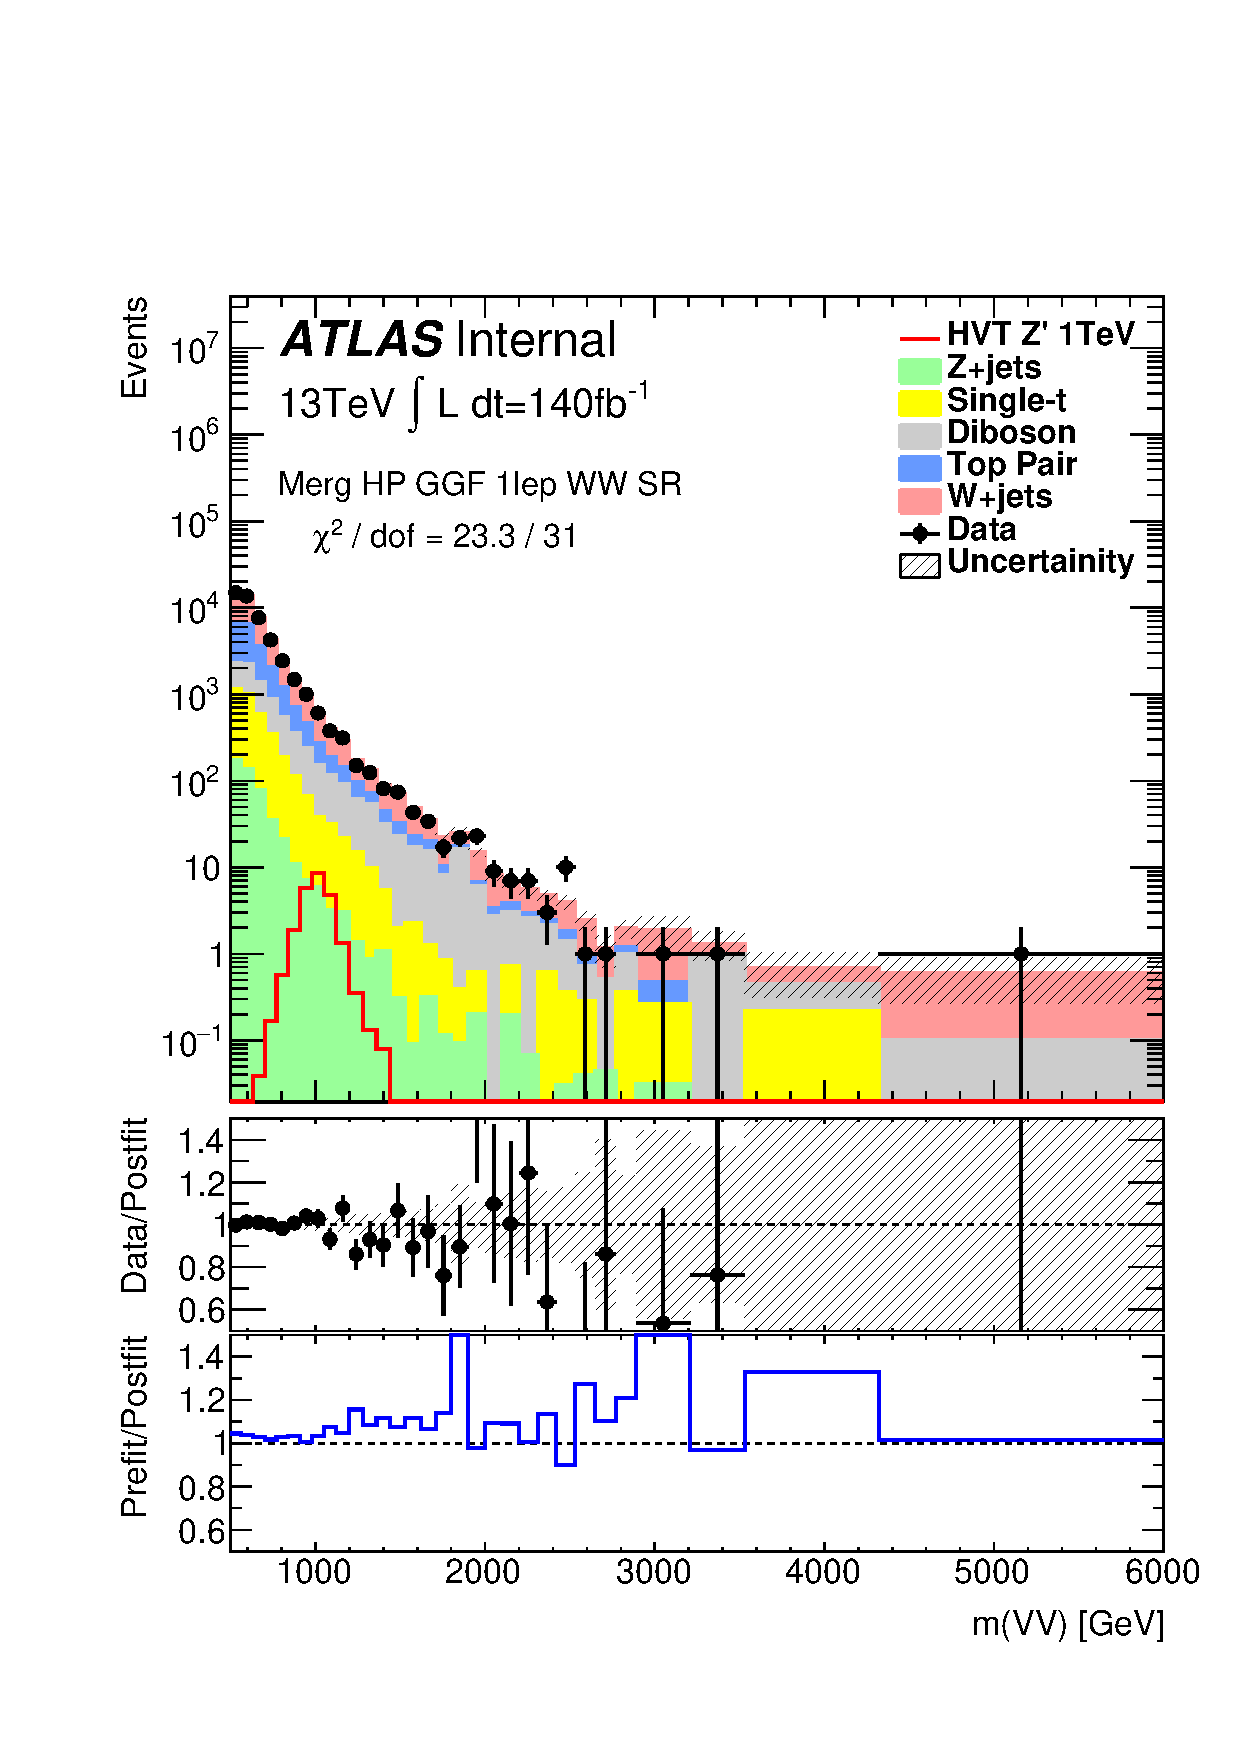
\includegraphics[width=0.3\hsize]{figures/results/HVTWW/L1_MergHP_GGF_WW_SR.pdf}
    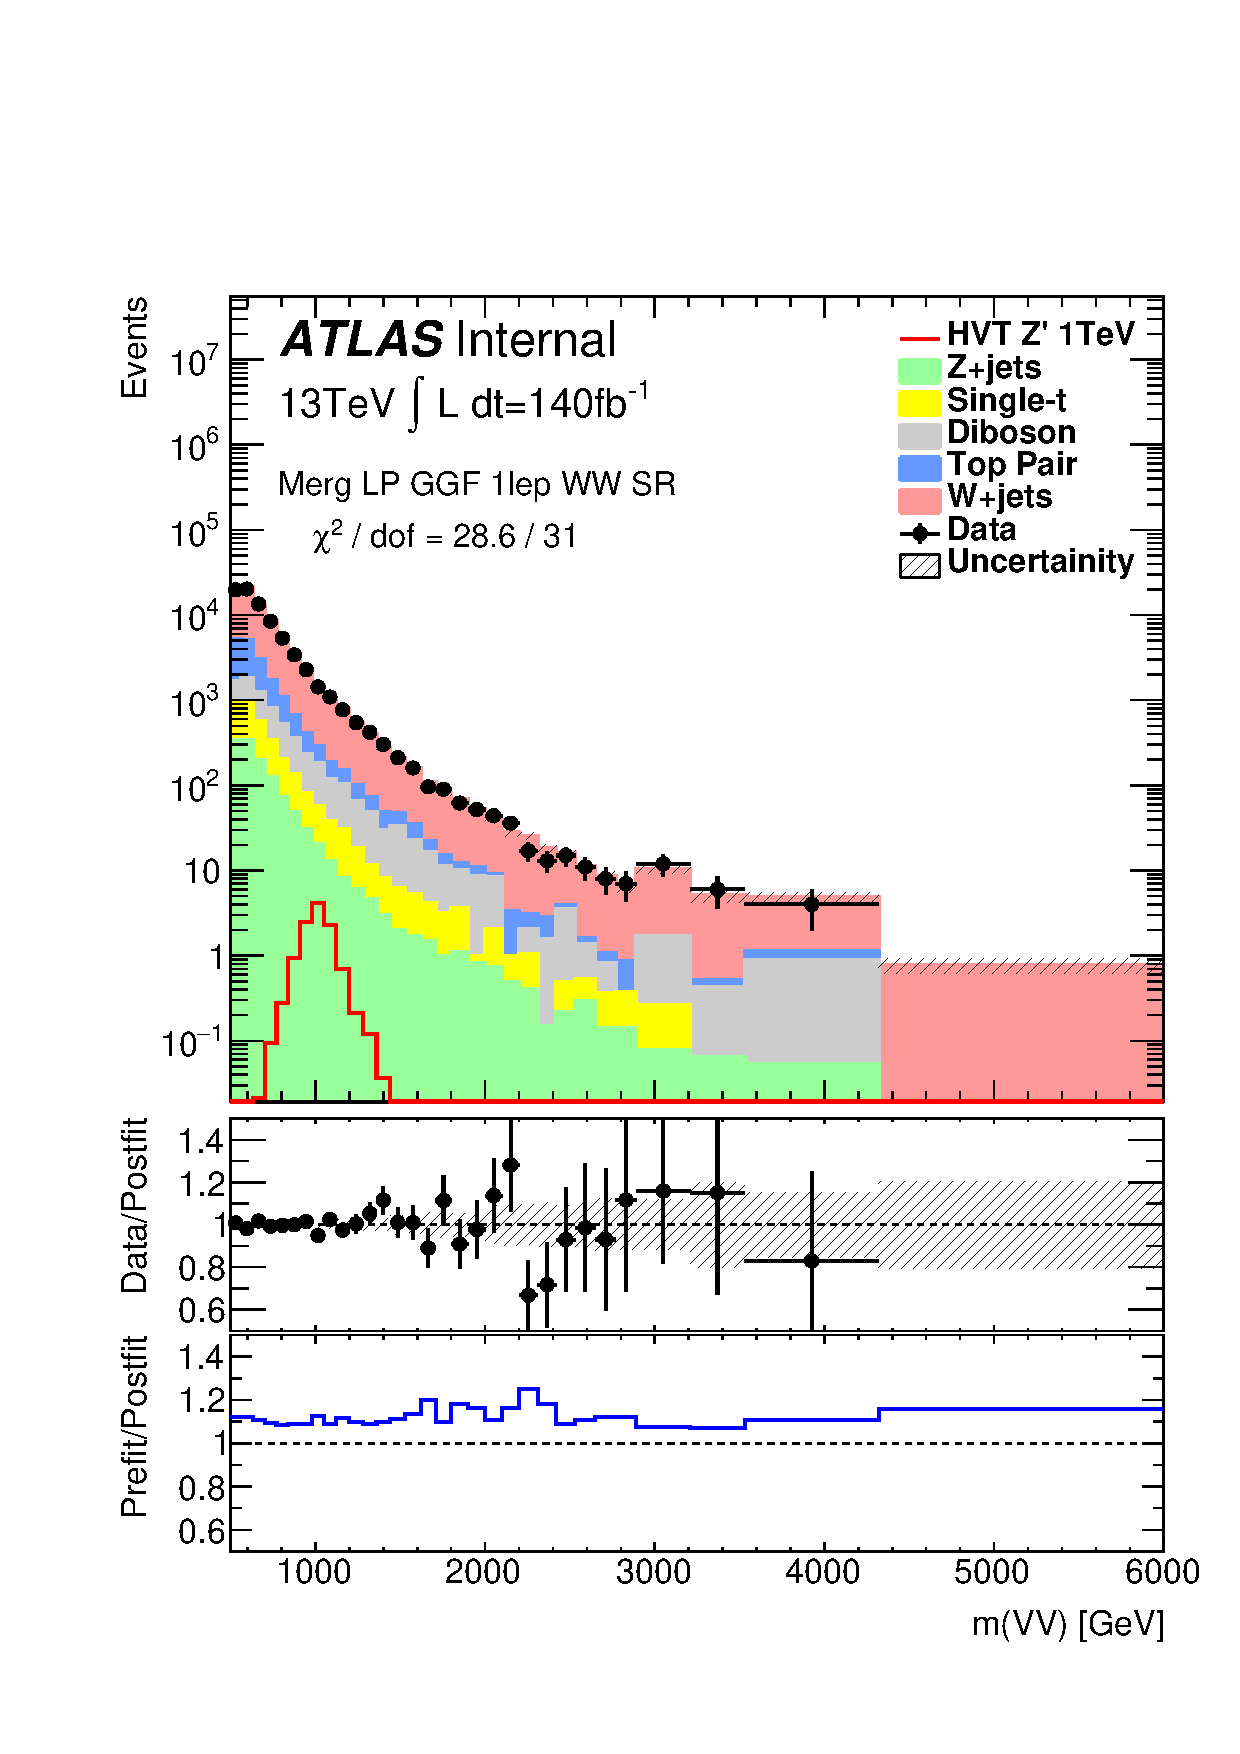
\includegraphics[width=0.3\hsize]{figures/results/HVTWW/L1_MergLP_GGF_WW_SR.pdf}
    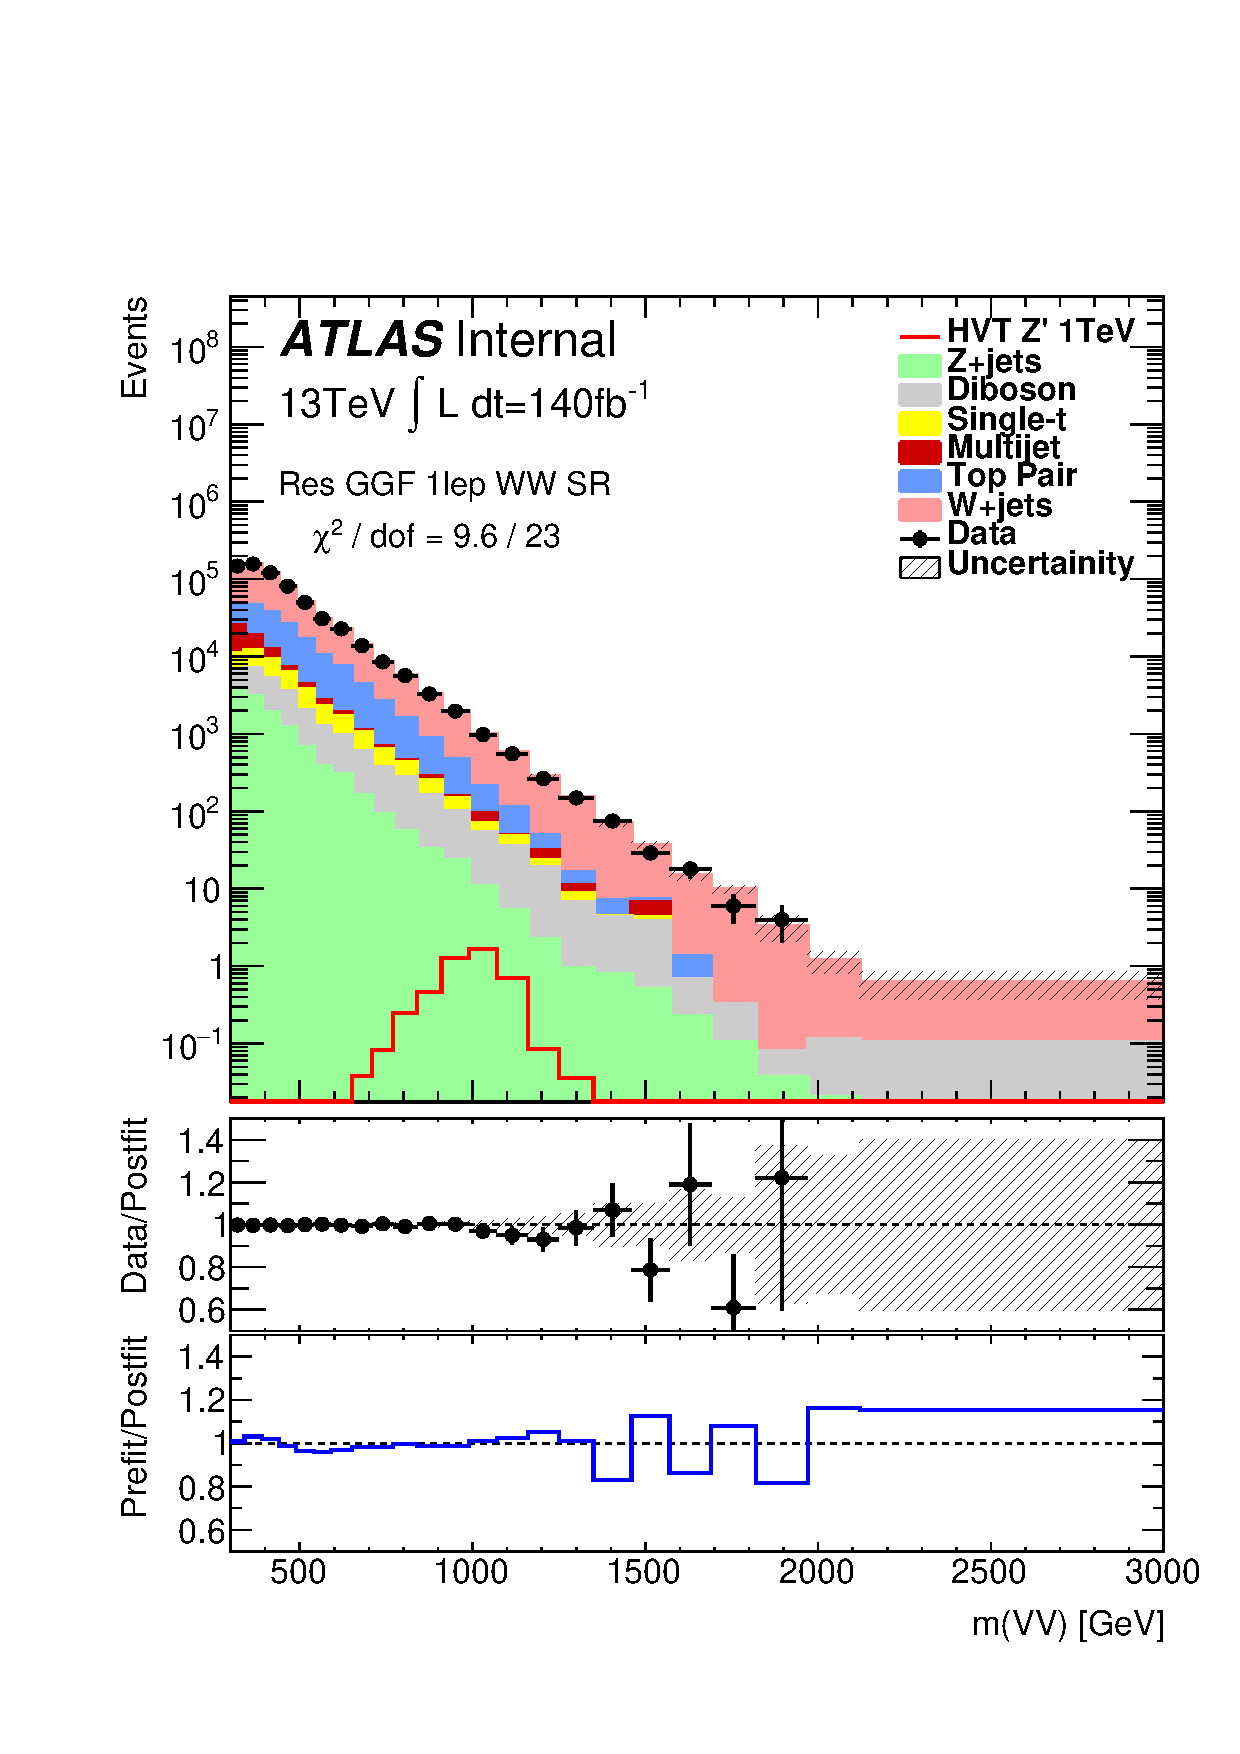
\includegraphics[width=0.3\hsize]{figures/results/HVTWW/L1_Res_GGF_WW_SR.pdf}
 \caption{The distribution of $m_{\ell\nu qq}$ in the non-VBF $WW$ signal regions.} 
  \label{fig:hvtww_sr_postfit}
\end{figure} 
\FloatBarrier

\begin{figure}[h!]
  \centering
  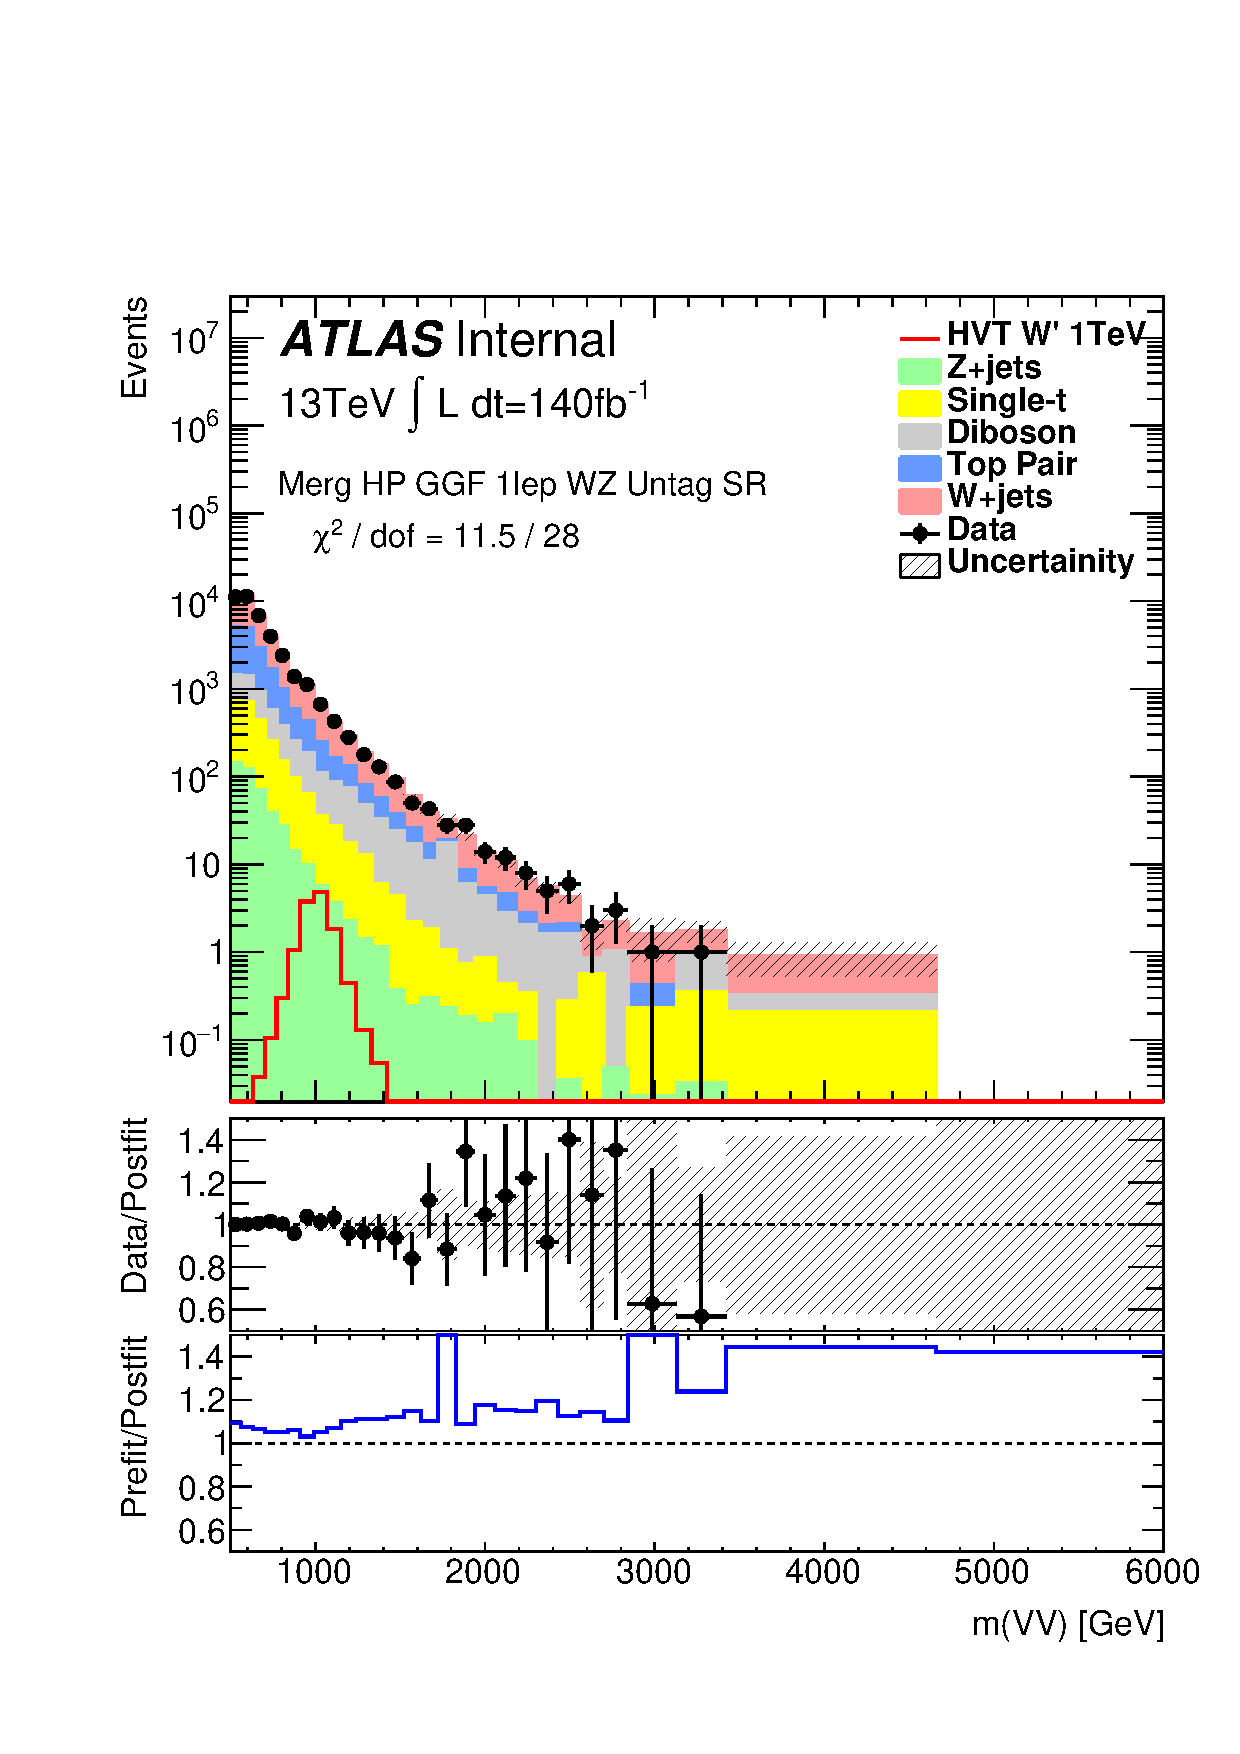
\includegraphics[width=0.3\hsize]{figures/results/HVTWZ/L1_MergHP_GGF_WZ_Untag_SR.pdf}
    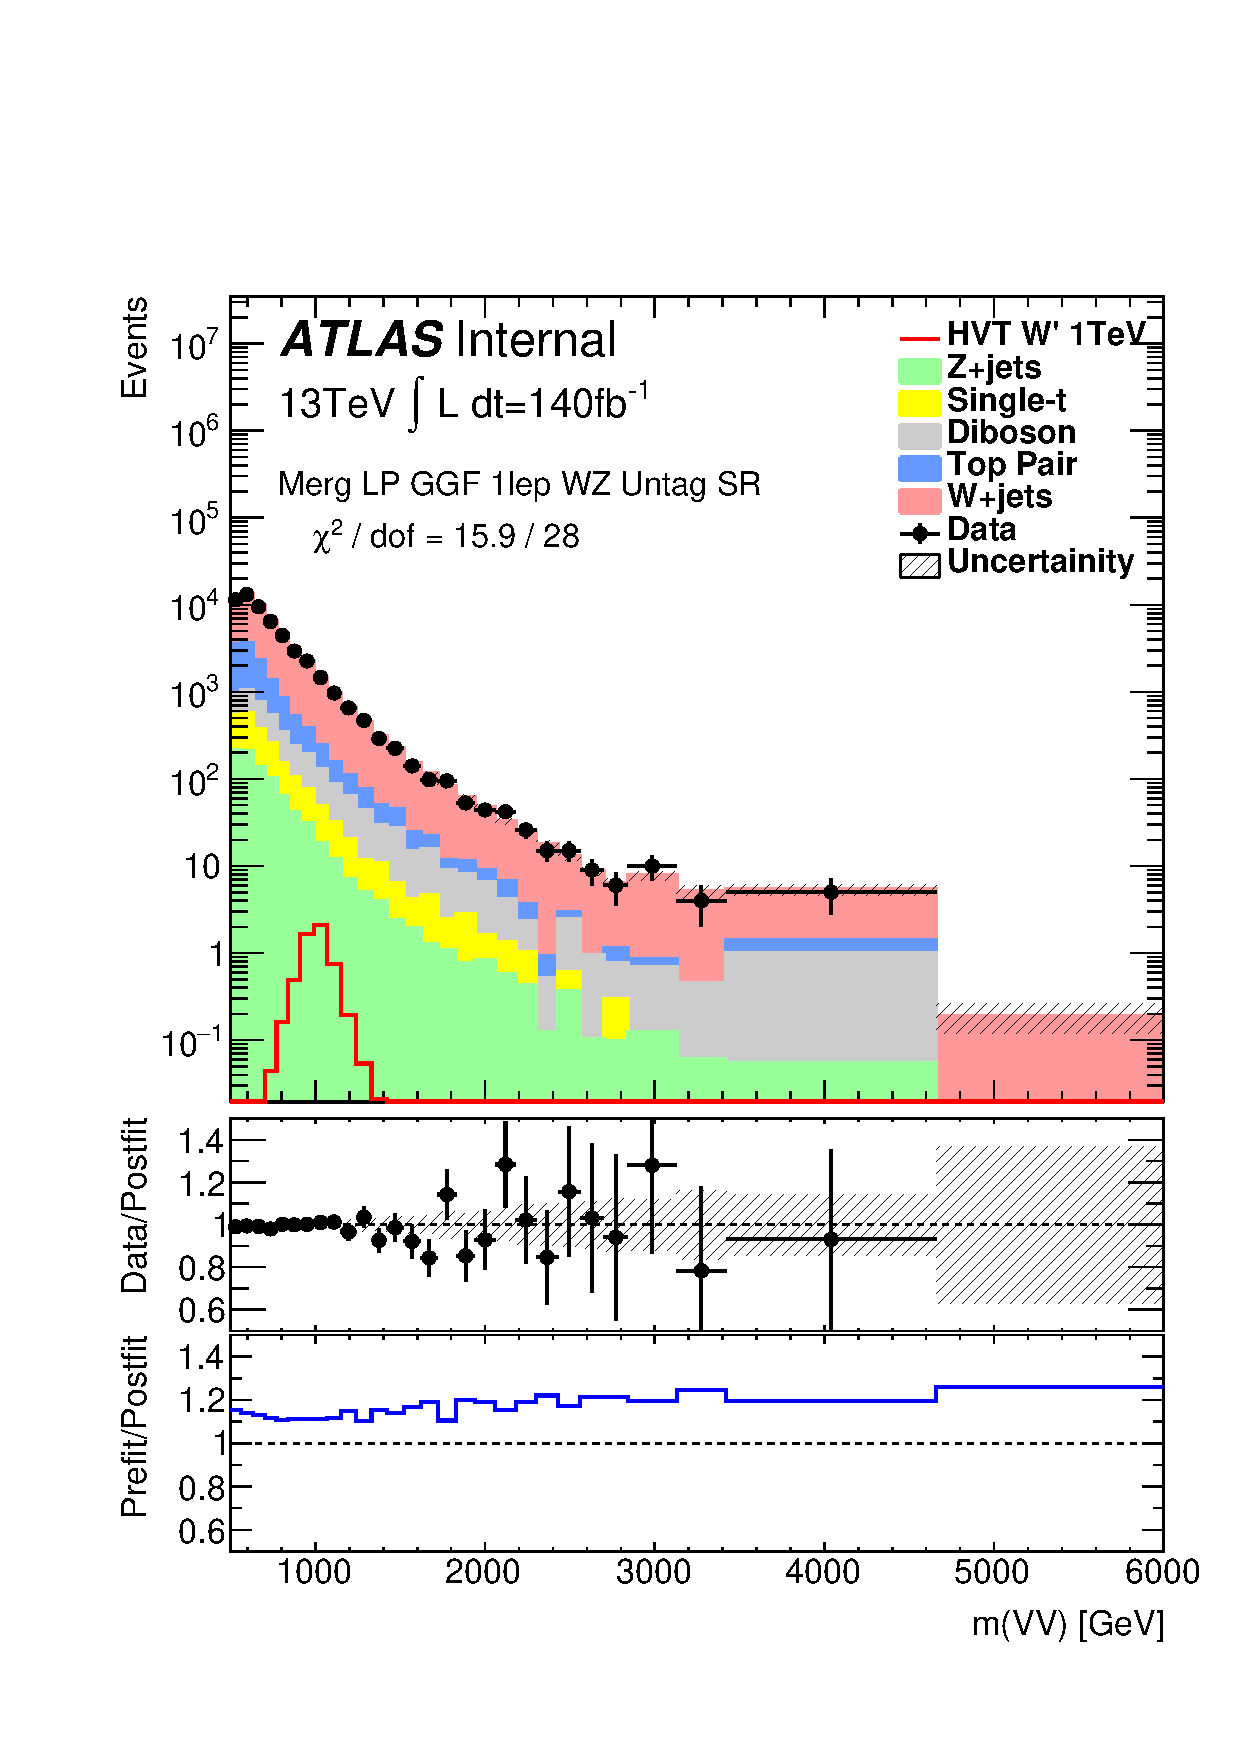
\includegraphics[width=0.3\hsize]{figures/results/HVTWZ/L1_MergLP_GGF_WZ_Untag_SR.pdf}
    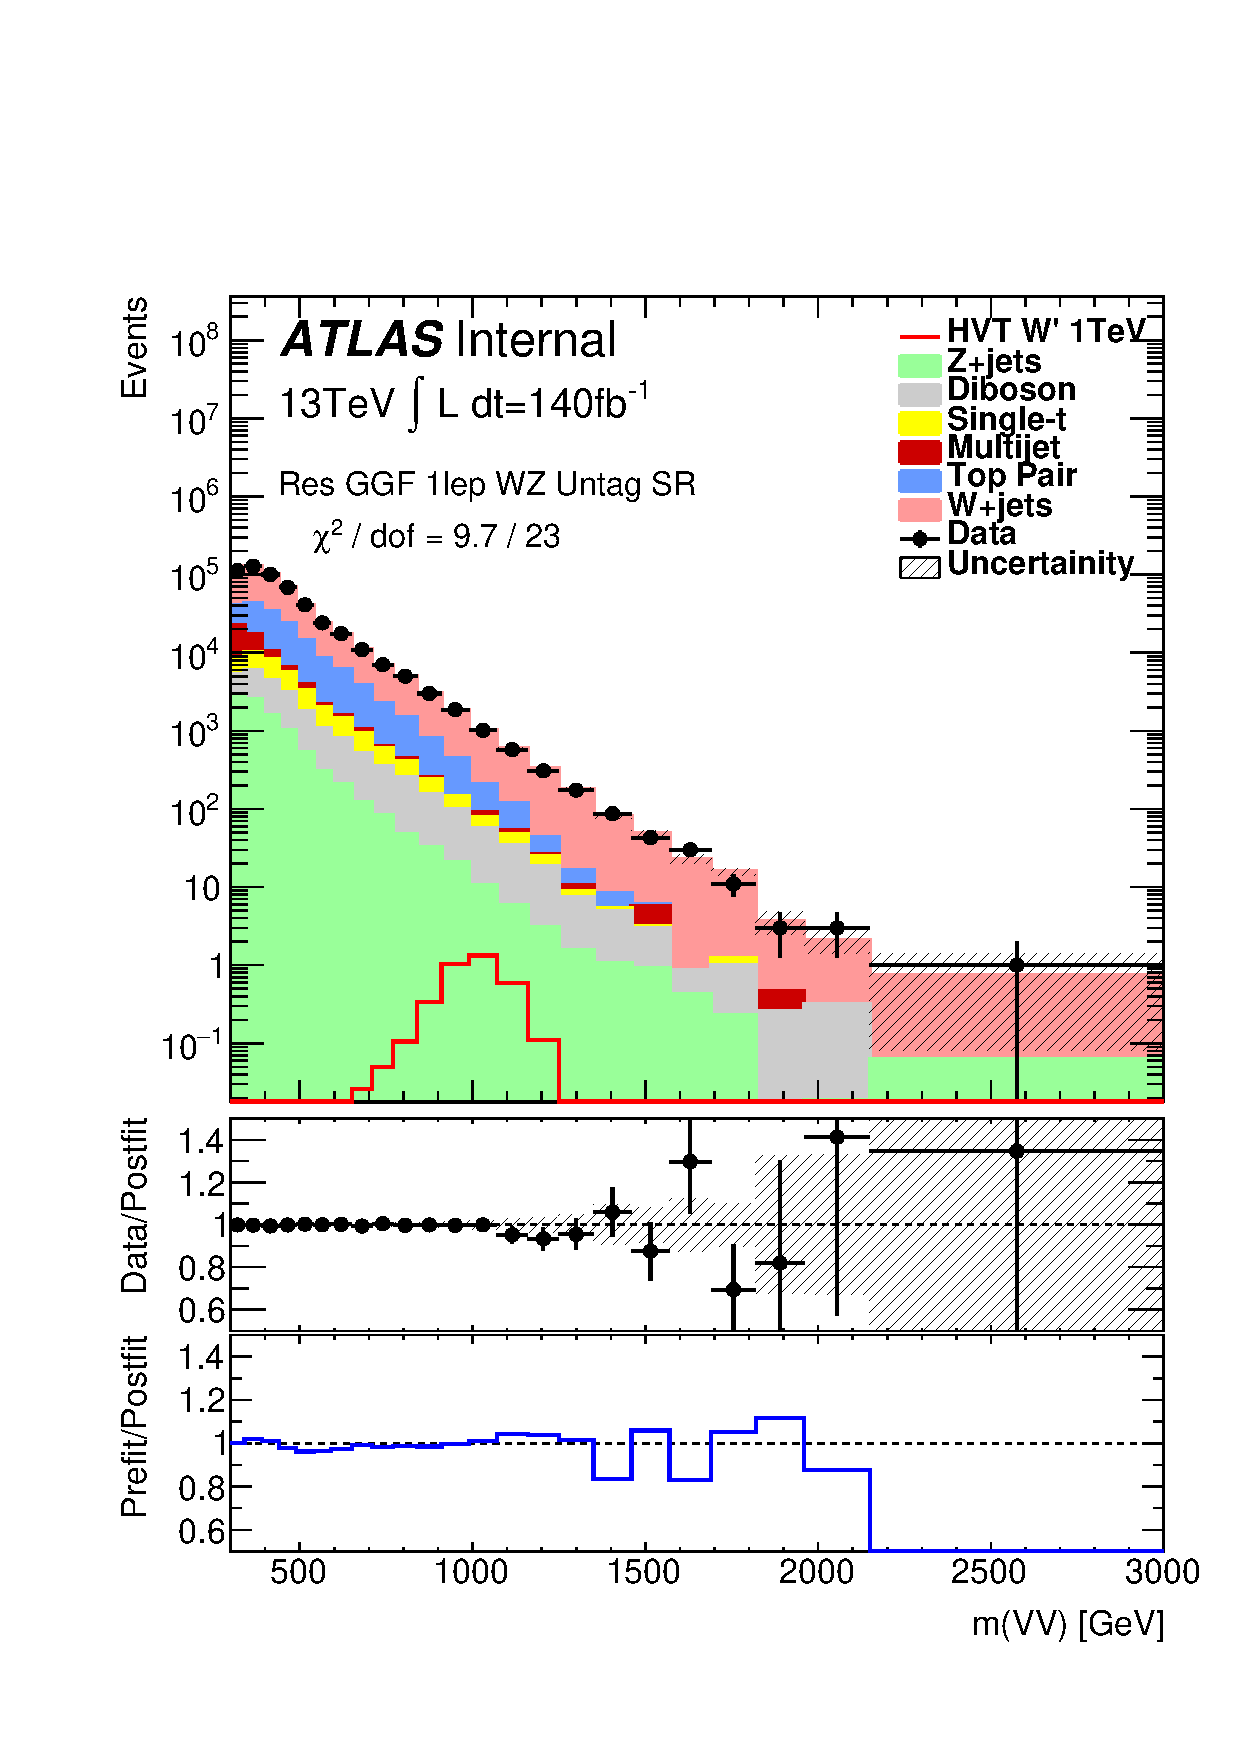
\includegraphics[width=0.3\hsize]{figures/results/HVTWZ/L1_Res_GGF_WZ_Untag_SR.pdf}
 \caption{The distribution of $m_{\ell\nu qq}$ in the non-VBF $WZ$ Untag signal regions.} 
  \label{fig:hvtwz_untag_sr_postfit}
\end{figure} 
\FloatBarrier

\begin{figure}[h!]
  \centering
  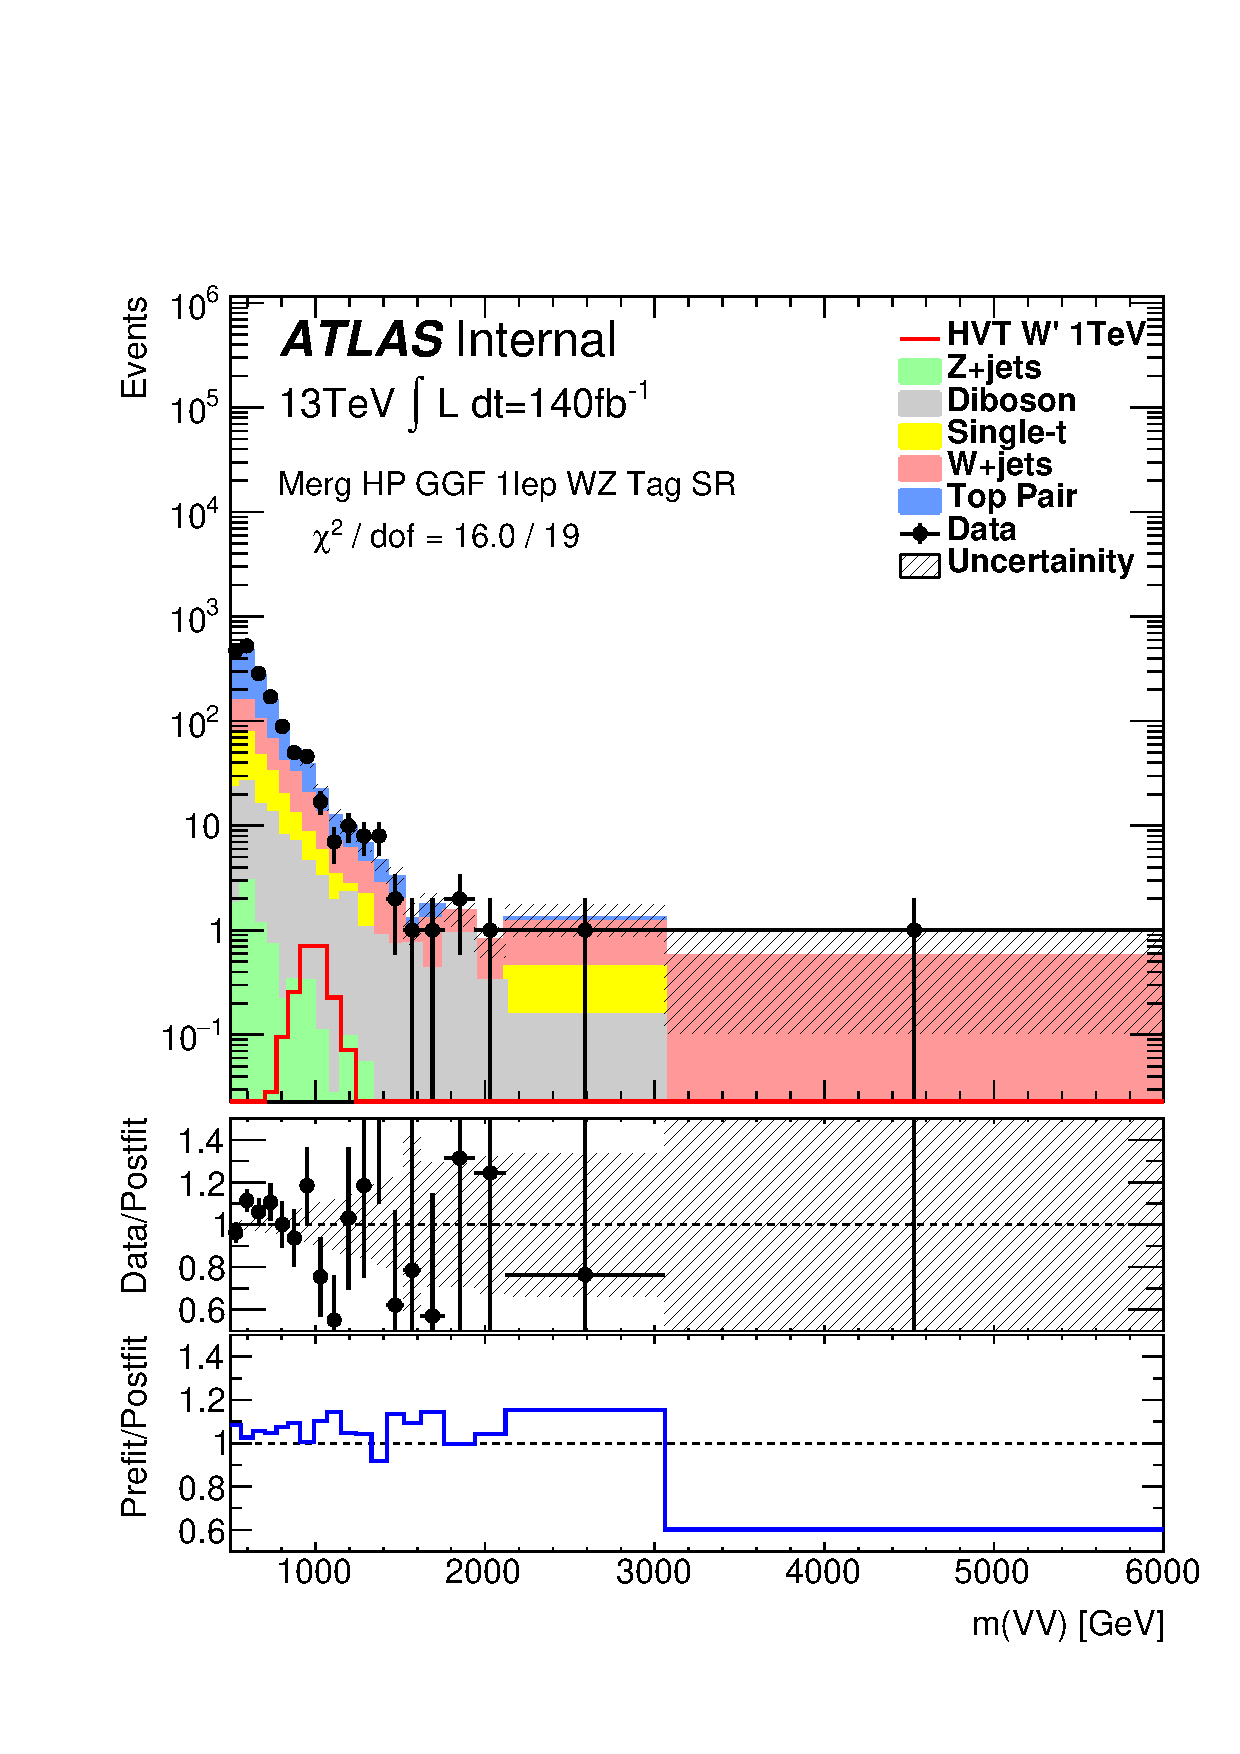
\includegraphics[width=0.3\hsize]{figures/results/HVTWZ/L1_MergHP_GGF_WZ_Tag_SR.pdf}
    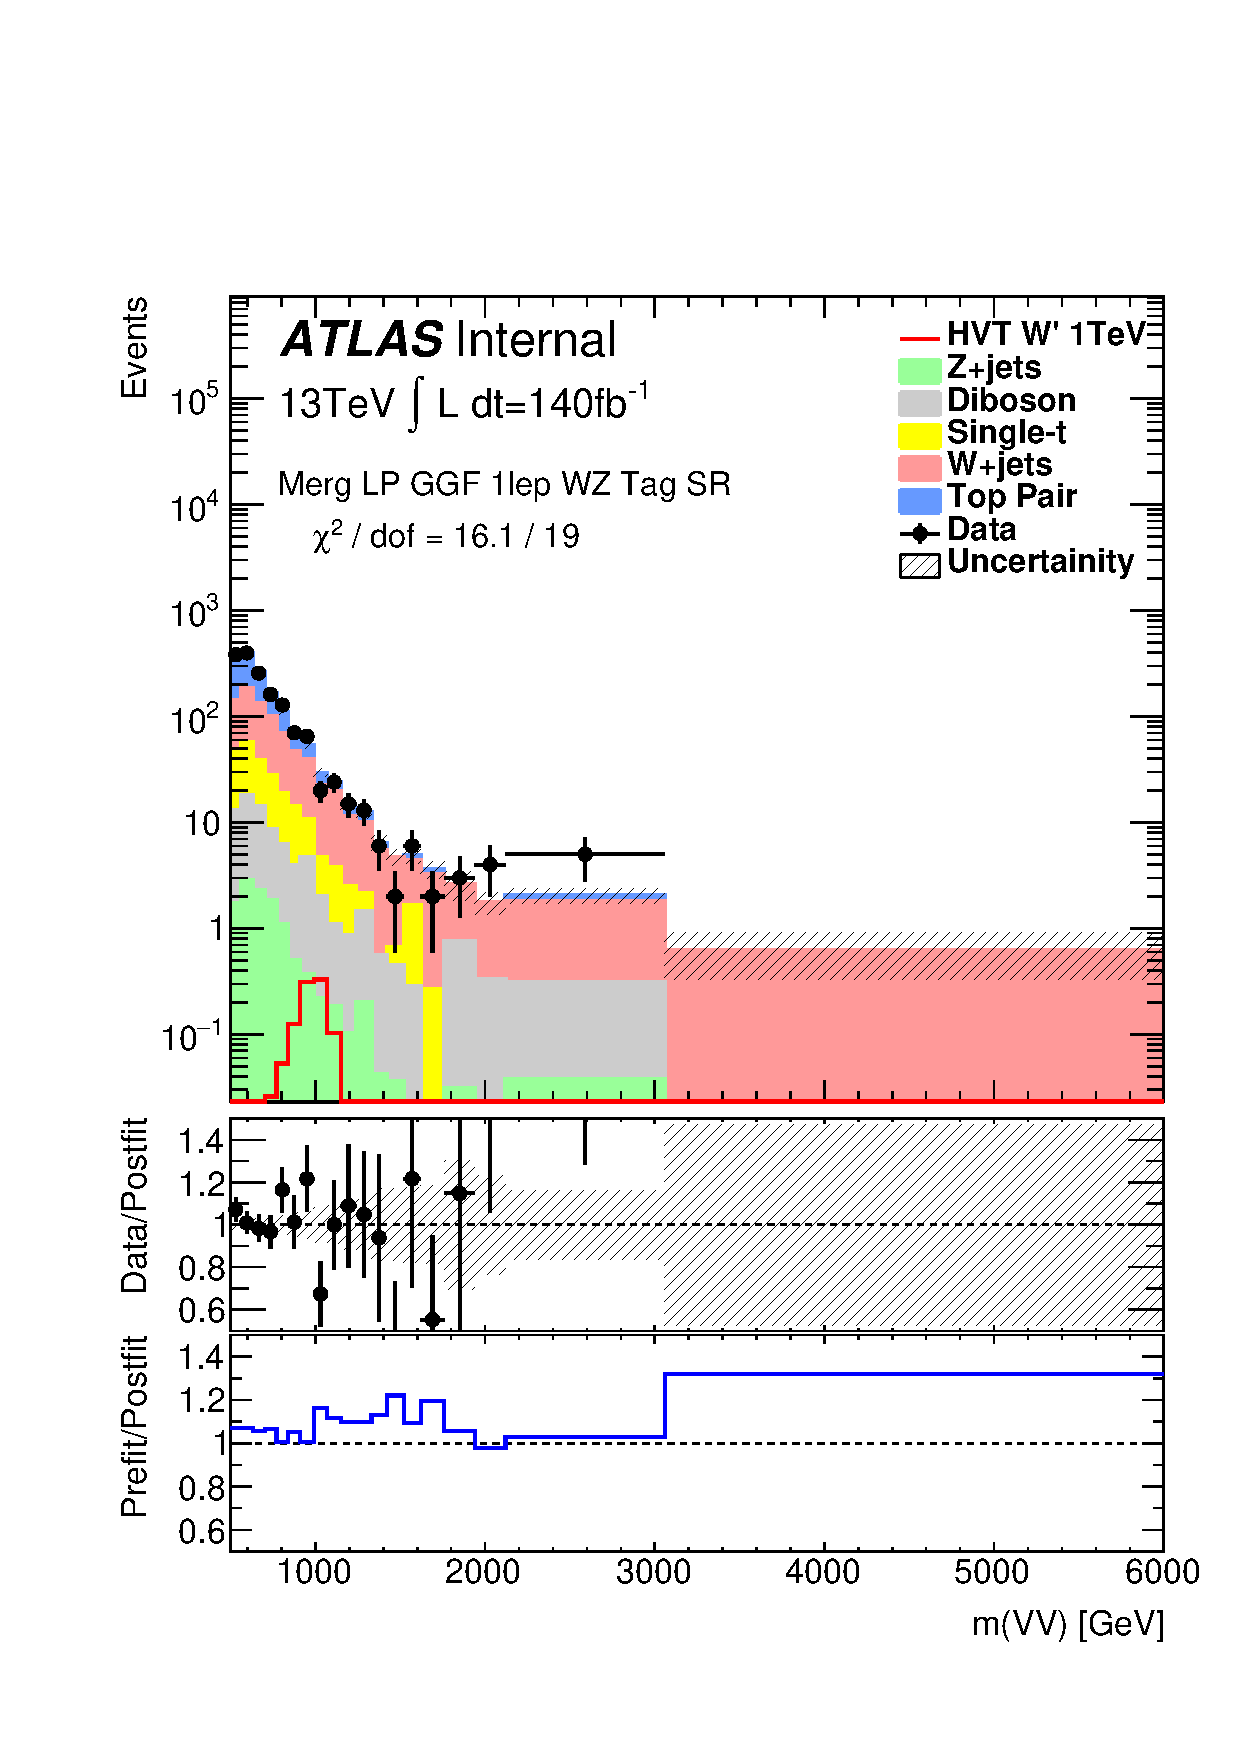
\includegraphics[width=0.3\hsize]{figures/results/HVTWZ/L1_MergLP_GGF_WZ_Tag_SR.pdf}
    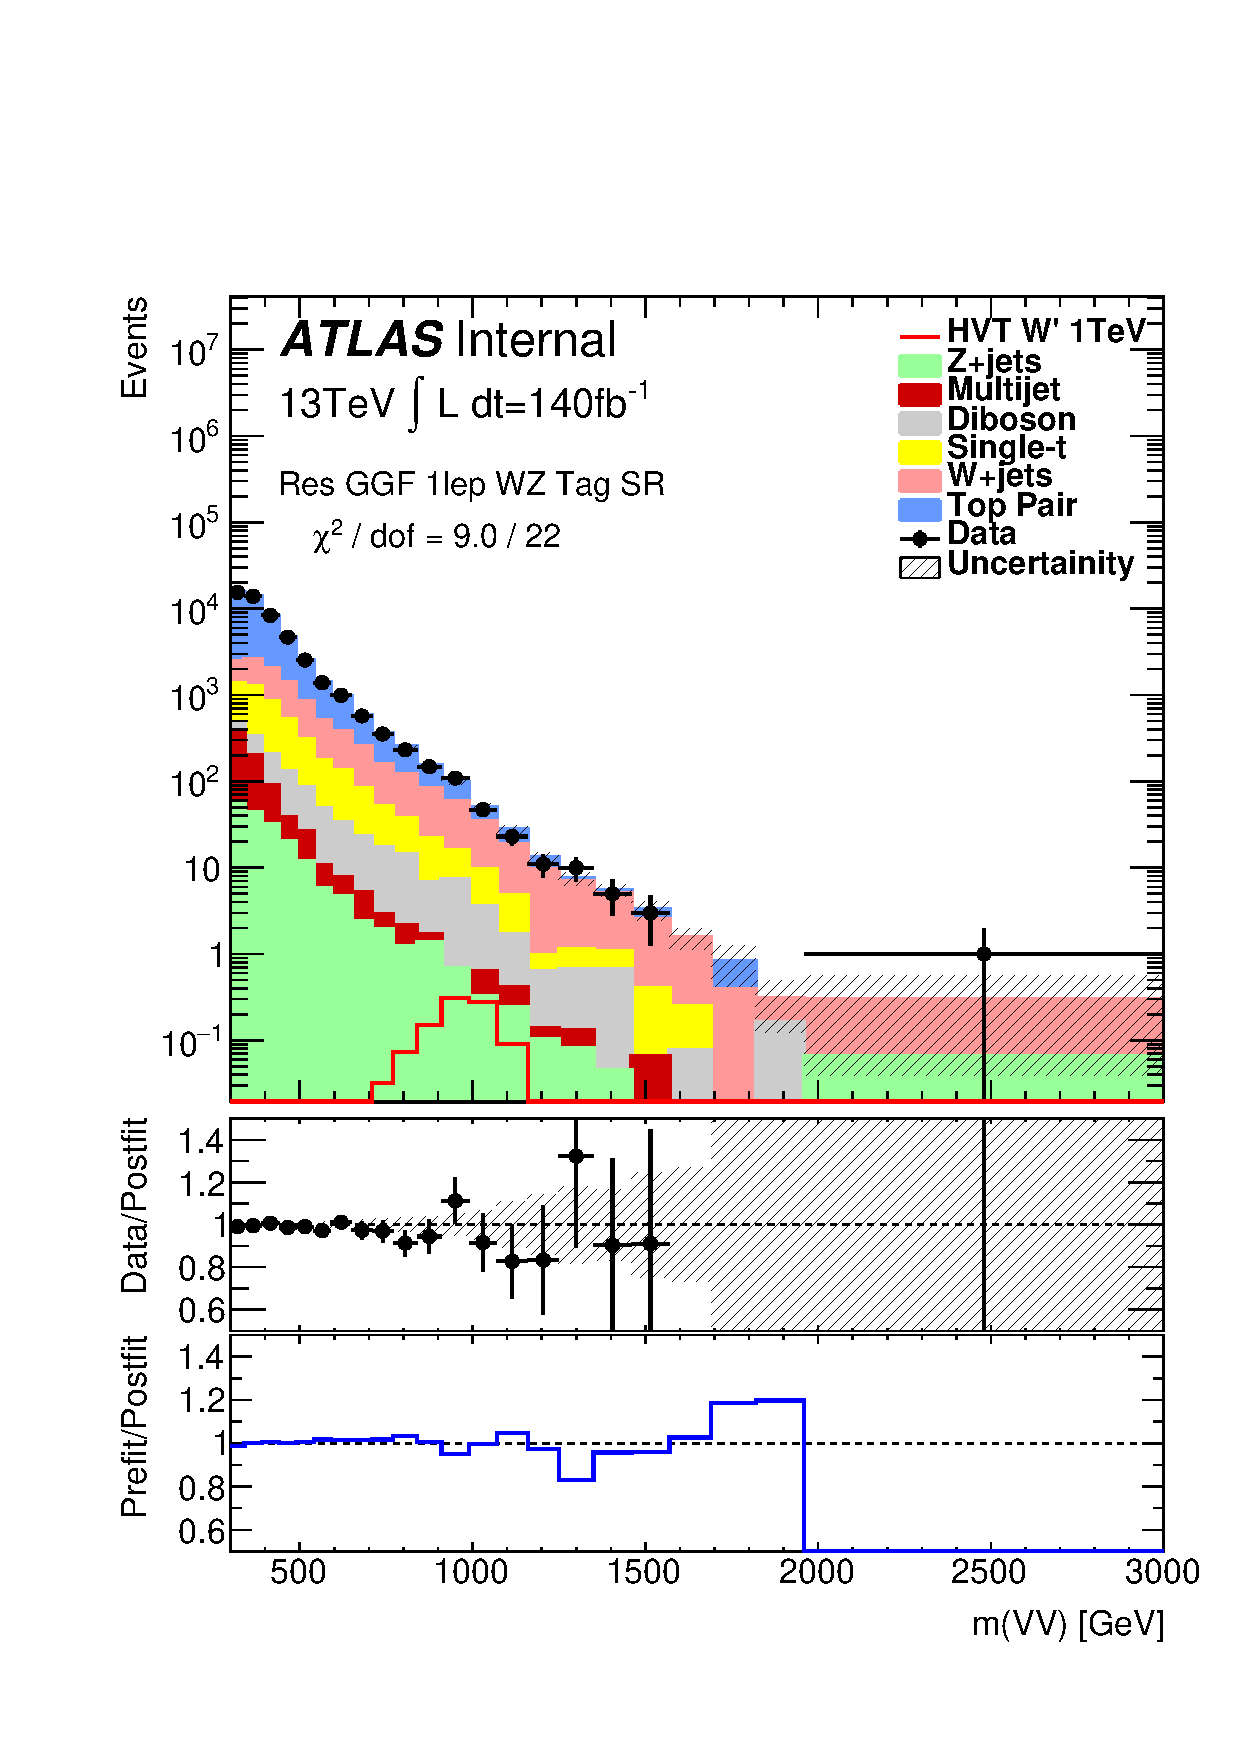
\includegraphics[width=0.3\hsize]{figures/results/HVTWZ/L1_Res_GGF_WZ_Tag_SR.pdf}
 \caption{The distribution of $m_{\ell\nu qq}$ in the non-VBF $WZ$ Tag signal regions.} 
  \label{fig:hvtwz_tag_sr_postfit}
\end{figure} 
\FloatBarrier

\begin{figure}[h!]
  \centering
  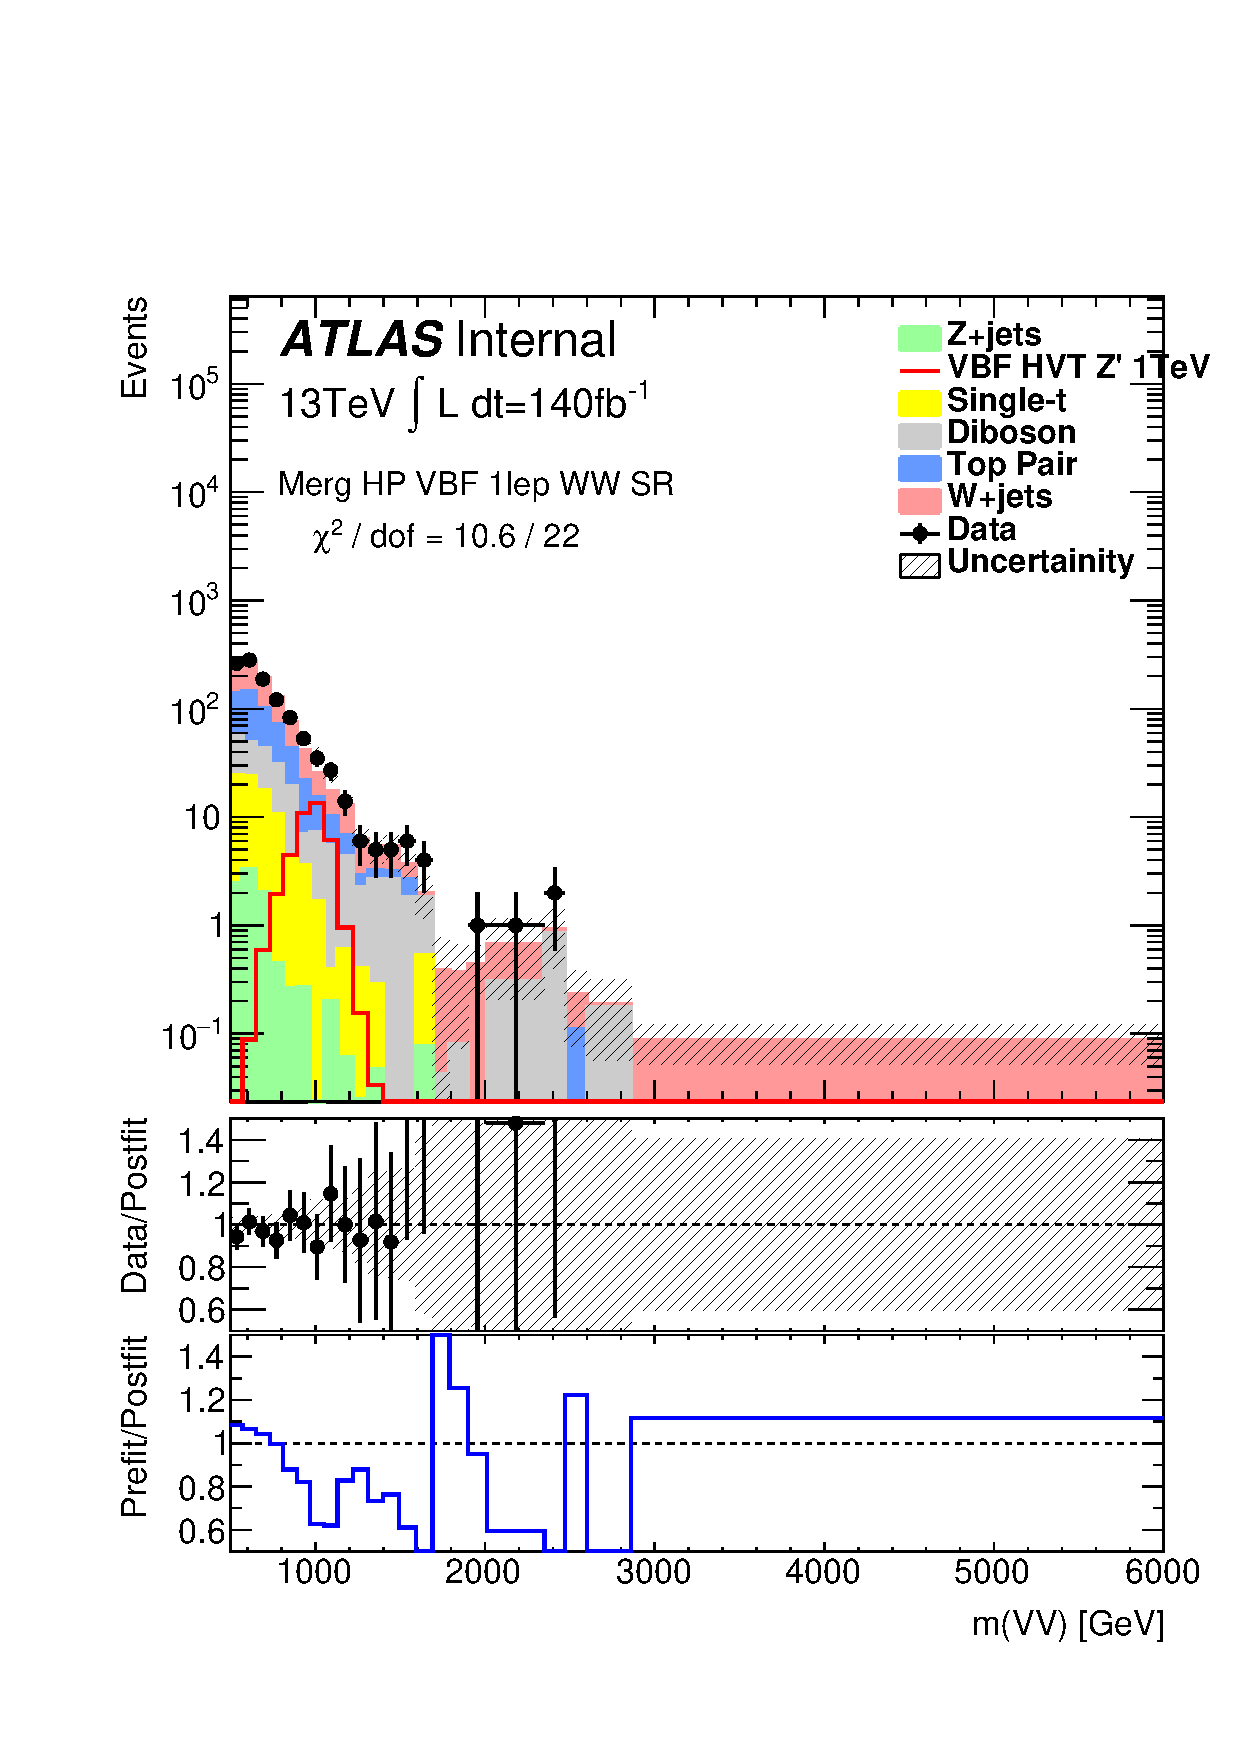
\includegraphics[width=0.3\hsize]{figures/results/HVTWWVBF/L1_MergHP_VBF_WW_SR.pdf}
    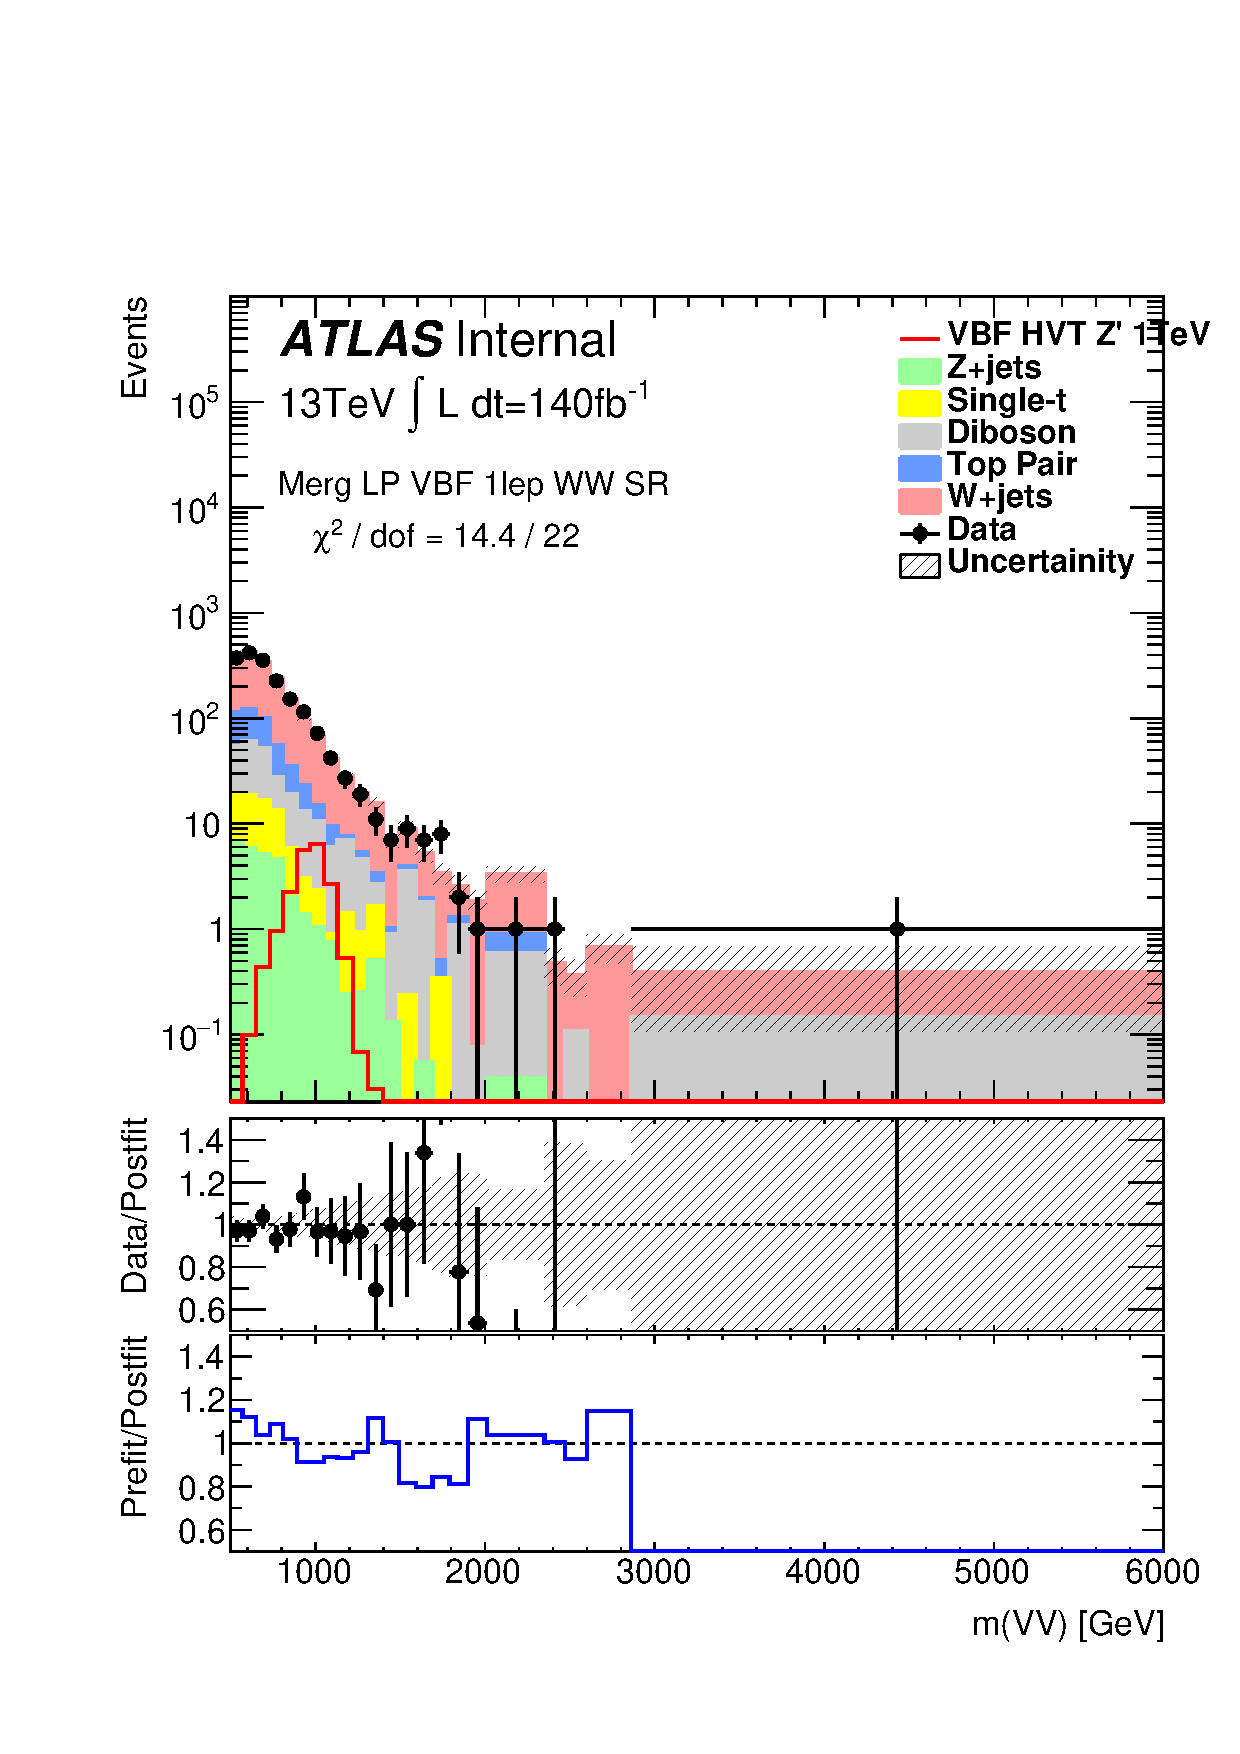
\includegraphics[width=0.3\hsize]{figures/results/HVTWWVBF/L1_MergLP_VBF_WW_SR.pdf}
    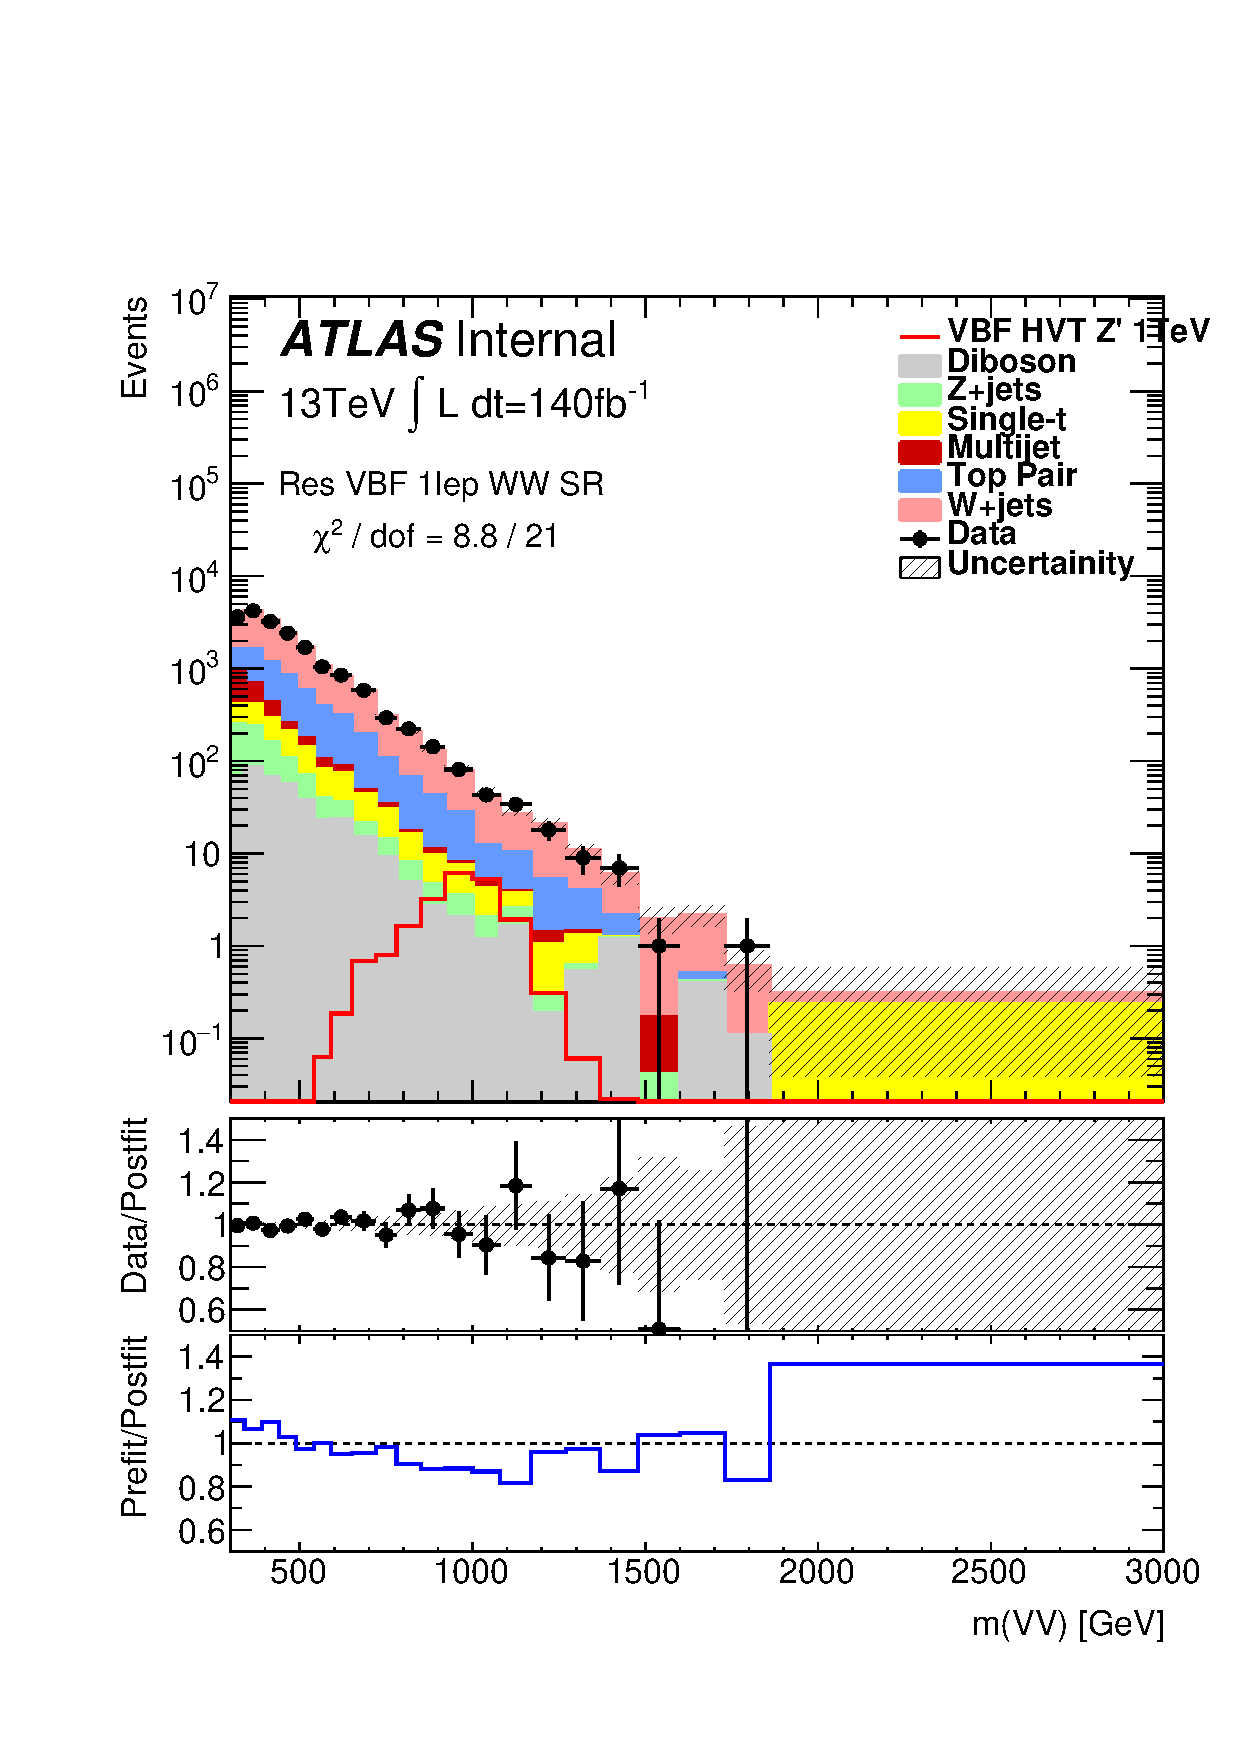
\includegraphics[width=0.3\hsize]{figures/results/HVTWWVBF/L1_Res_VBF_WW_SR.pdf}
 \caption{The distribution of $m_{\ell\nu qq}$ in the VBF $WZ$ Tag signal regions.} 
  \label{fig:hvtwwvbf_tag_sr_postfit}
\end{figure} 
\FloatBarrier

\begin{figure}[h!]
  \centering
  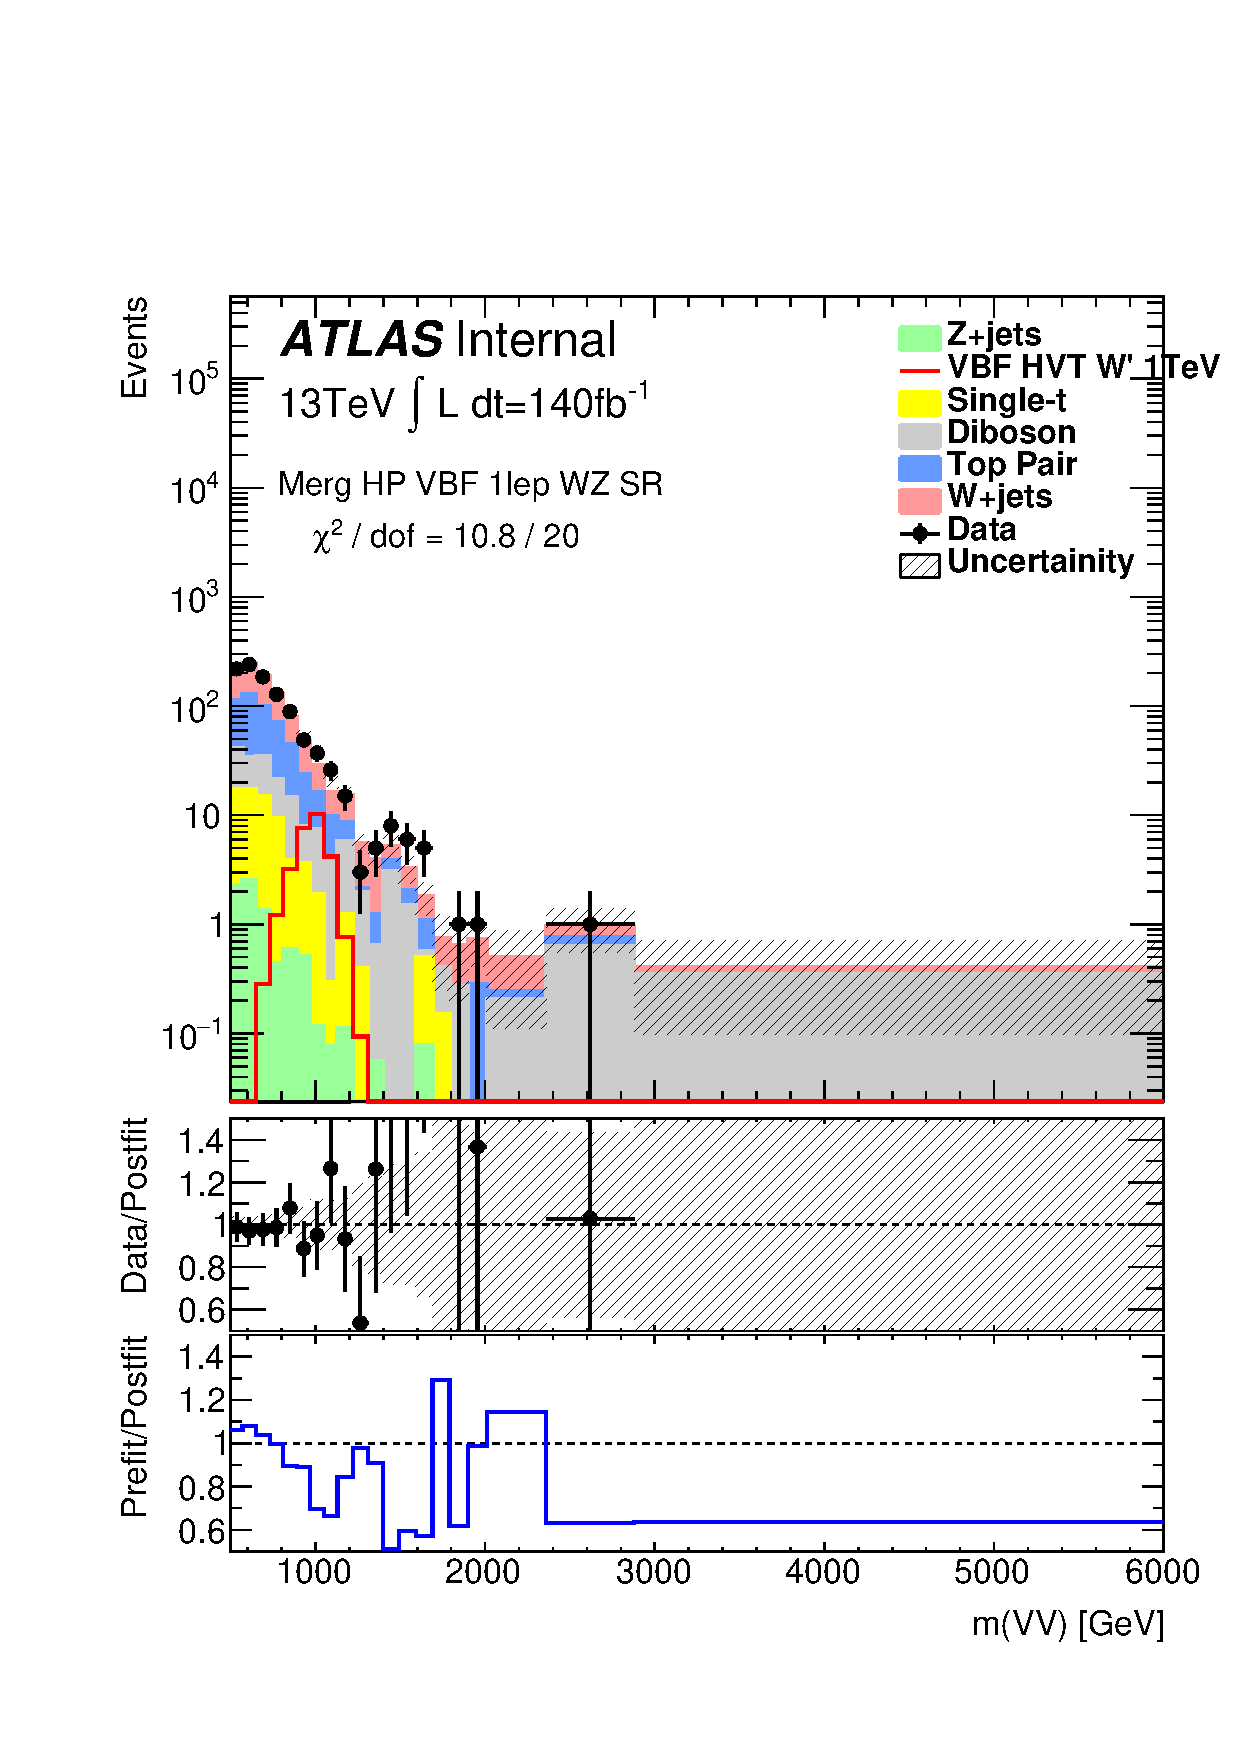
\includegraphics[width=0.3\hsize]{figures/results/HVTWZVBF/L1_MergHP_VBF_WZ_SR.pdf}
    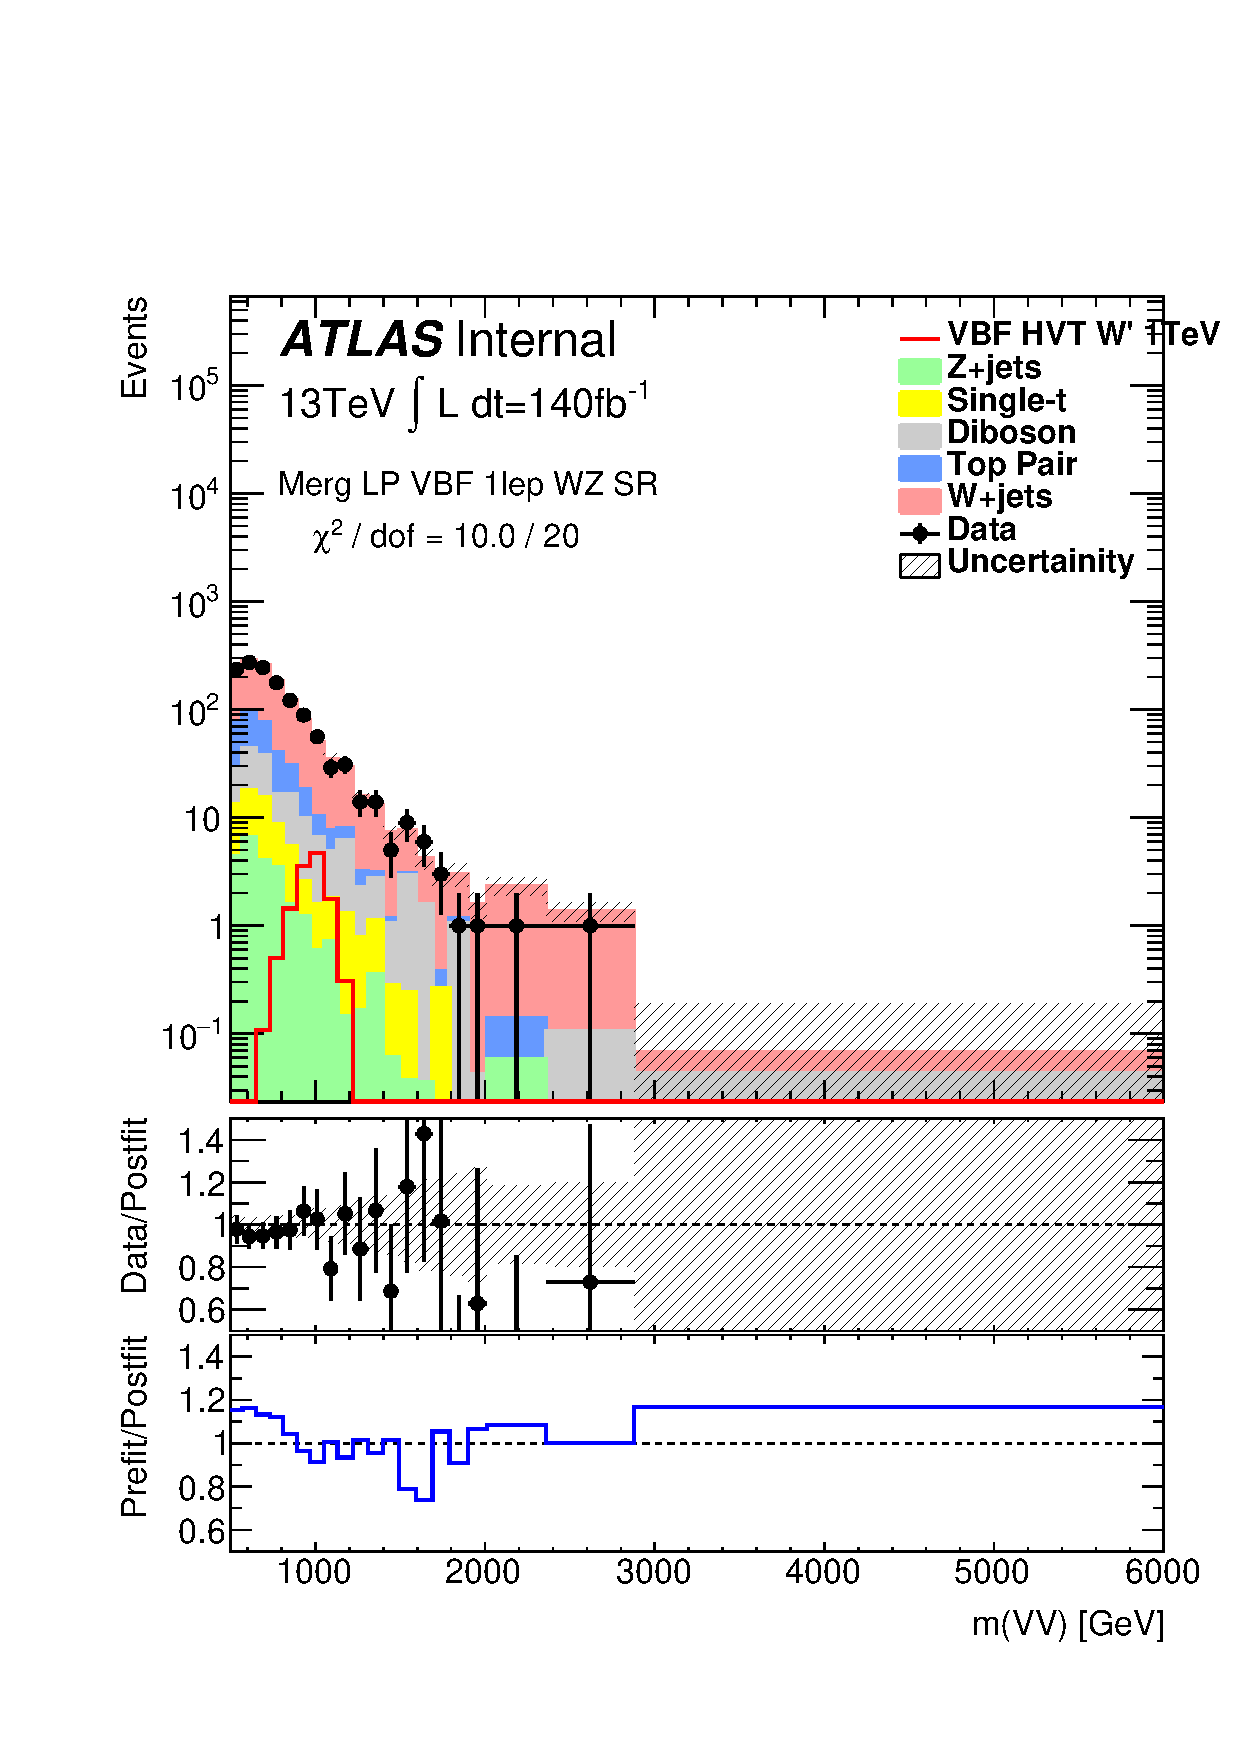
\includegraphics[width=0.3\hsize]{figures/results/HVTWZVBF/L1_MergLP_VBF_WZ_SR.pdf}
    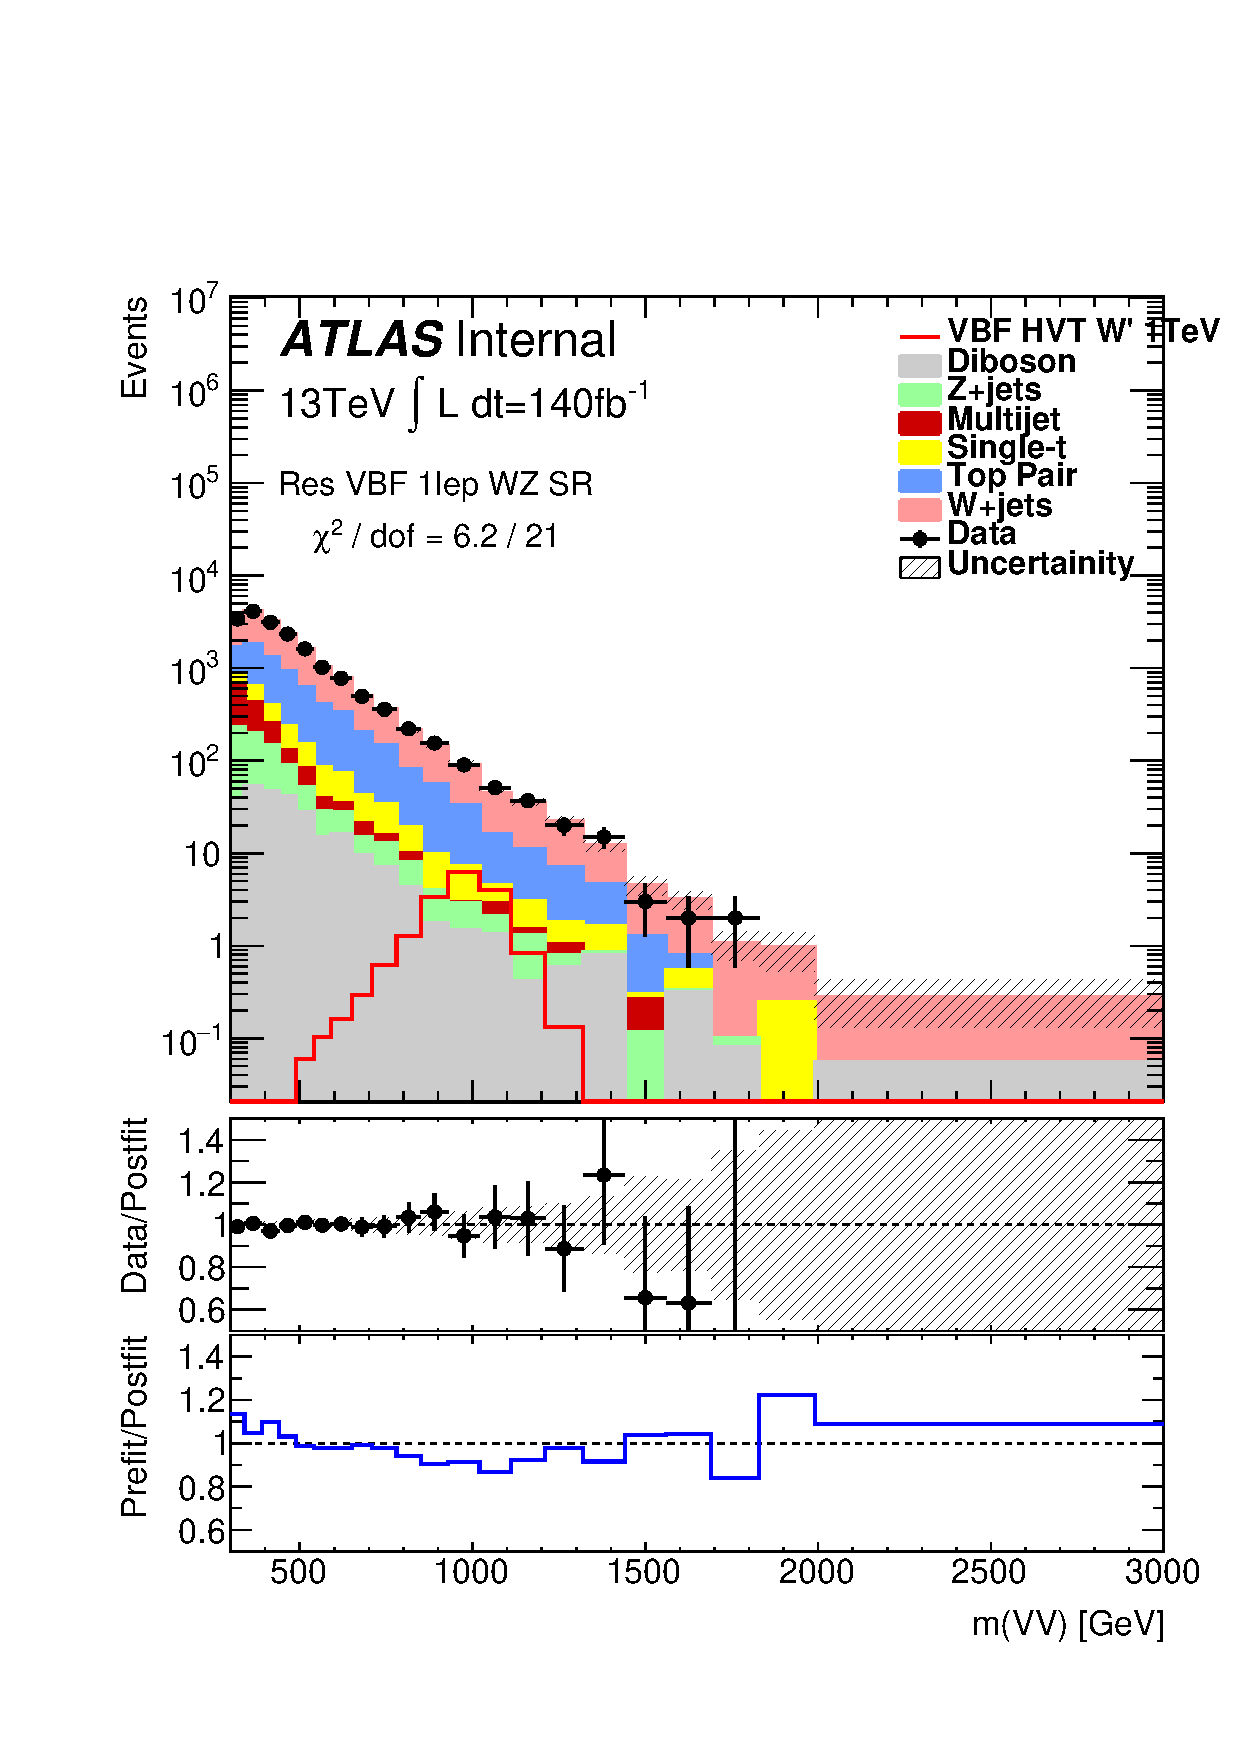
\includegraphics[width=0.3\hsize]{figures/results/HVTWZVBF/L1_Res_VBF_WZ_SR.pdf}
 \caption{The distribution of $m_{\ell\nu qq}$ in the VBF $WZ$ Tag signal regions.} 
  \label{fig:hvtwzvbf_tag_sr_postfit}
\end{figure} 
\FloatBarrier

\section{Systematic Profiling and Correlations}
The ranked systematics and their fitted values are shown for the different analysis regions in Figure \ref{fig:hvtww_ranking} - \ref{fig:hvtwz_ranking}. Note that background normalizations for $W$+jets and $t\bar{t}$ are left free to float in the fit. This means the nominal normalization values are at one and the uncertainties are not shown in the ranked plots. Overall, systematics are not pulled outside their uncertainties, especially nuisance parameters that affect the fitted $\mu$ value most significantly. 

The correlation between systematics are shown in Figure \ref{fig:hvtww_corr}. Correlations between background normalization are expected. The remaining systematic correlations are not very strong or unexpected.
\begin{figure}[h!]
  \centering
  \includegraphics[width=0.48\hsize]{figures/results/HVTWW/ranking_data/nov7_hvtww_2000gev/ranking.pdf}
    \includegraphics[width=0.48\hsize]{figures/results/HVTWWVBF/ranking_data/nov7_hvtwwvbf_1000gev/ranking.pdf}
 \caption{Ranked systematics and their fitted values for $WW$ non-VBF (right) and VBF (left) selections.} 
  \label{fig:hvtww_ranking}
\end{figure} 
\FloatBarrier

\begin{figure}[h!]
  \centering
  \includegraphics[width=0.48\hsize]{figures/results/HVTWZ/ranking_data/nov7_hvtwz_1000gev/ranking.pdf}
    \includegraphics[width=0.48\hsize]{figures/results/HVTWZVBF/ranking_data/nov7_hvtwzvbf_1000gev/ranking.pdf}
 \caption{Ranked systematics and their fitted values for $WZ$ non-VBF (right) and VBF (left) selections.} 
  \label{fig:hvtwz_ranking}
\end{figure} 
\FloatBarrier

\begin{figure}[h!]
  \centering
  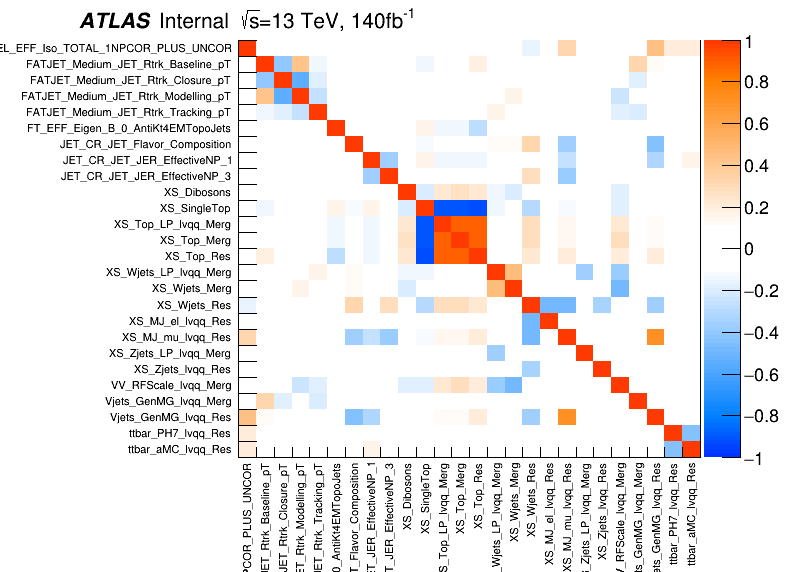
\includegraphics[width=0.48\hsize]{figures/Results/HVTWW/HVTWW_combined_1nov8_maybeFloatRelevantUncorrXSSingleBinPrunSyst/Plots/CorrMatrix/corr_doAsimov0_doCondtional1_mu0_HighCorr.png}
   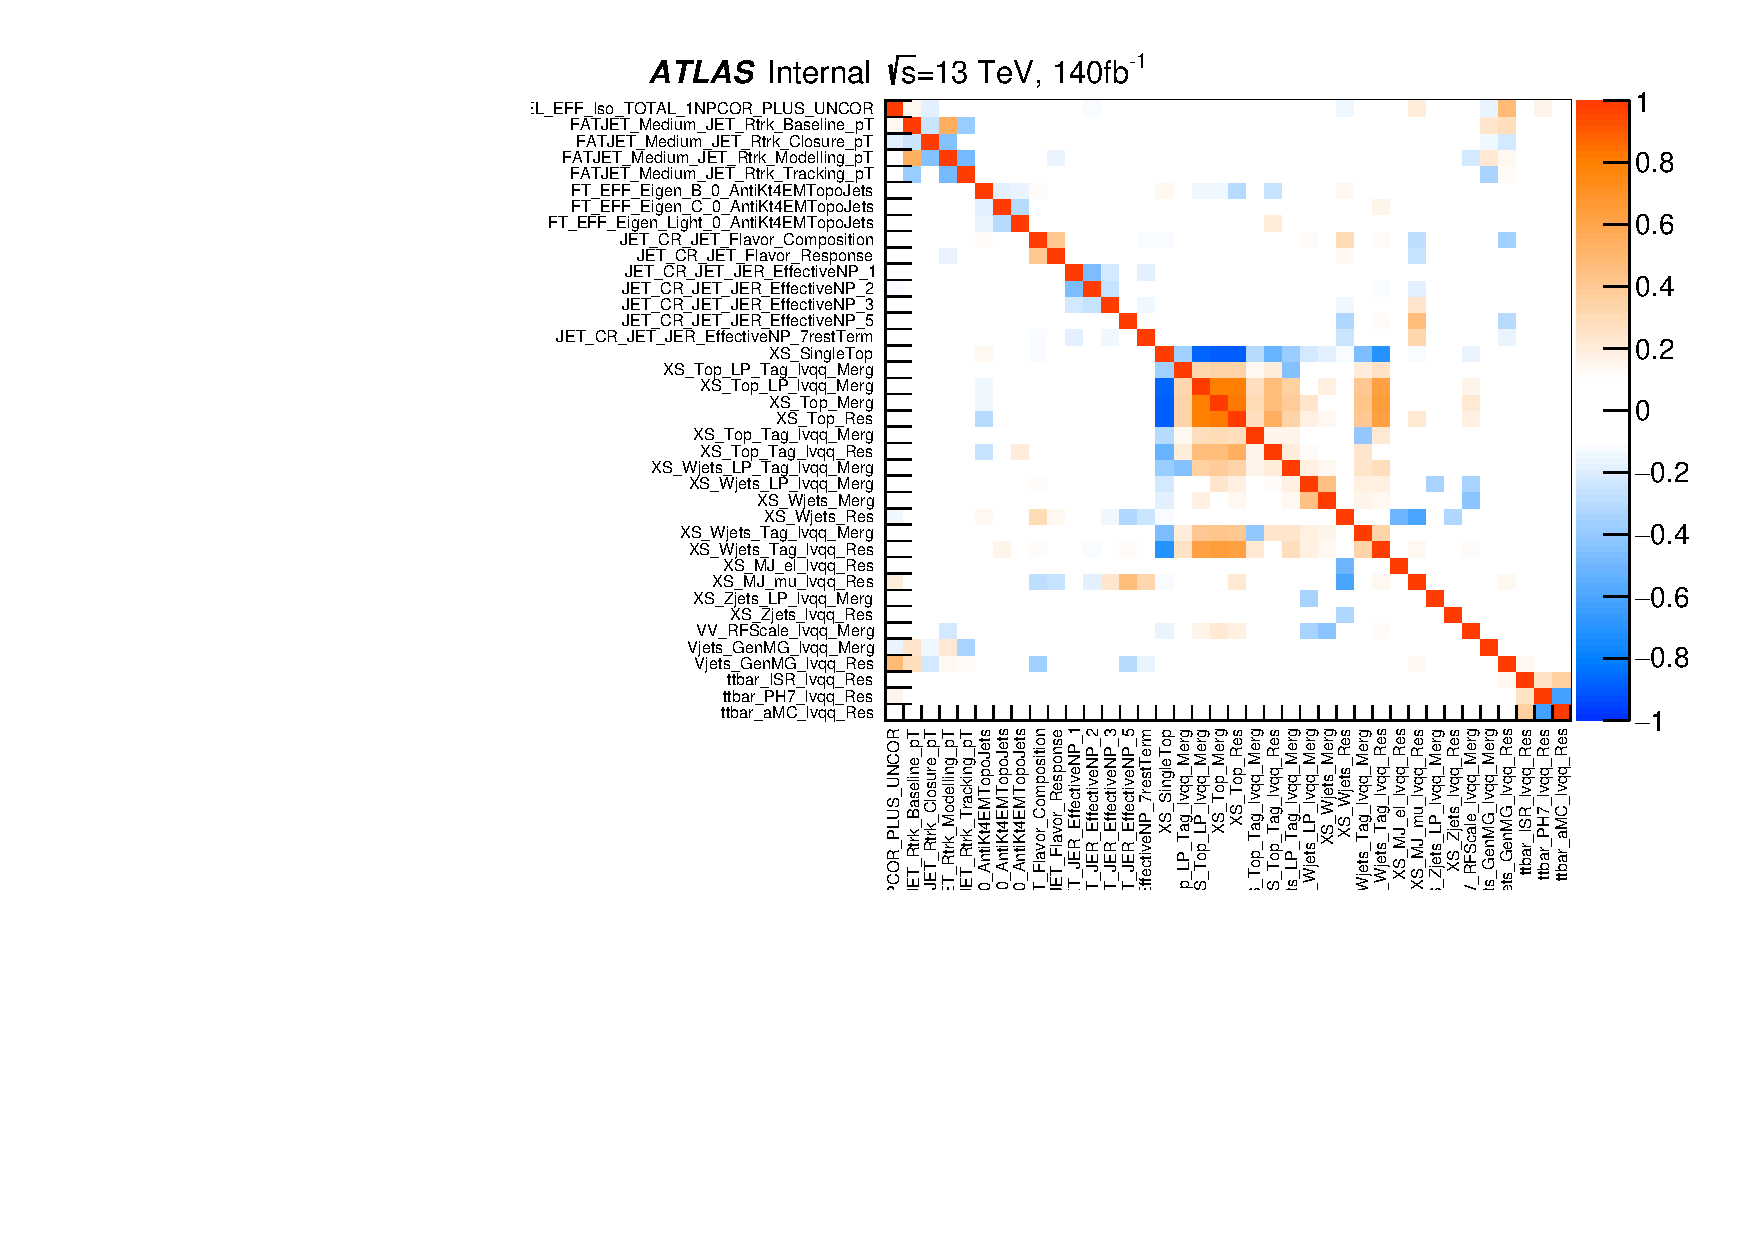
\includegraphics[width=0.48\hsize]{figures/Results/HVTWWVBF/HVTWWVBF_combined_1nov8_maybeFloatRelevantUncorrXSSingleBinPrunSyst/Plots/CorrMatrix/corr_doAsimov0_doCondtional1_mu0_HighCorr.pdf}
 \caption{Correlations between systematics for $WW$ non-VBF (right) and VBF (left) selections.} 
  \label{fig:hvtww_corr}
\end{figure} 
\FloatBarrier


\section{Discovery Tests}
To test for the existence of signal in the observed dataset, the discovery tests discussed earlier are used to calculate p-values as a function of resonance mass. The results of these tests are shown in Figures \ref{fig:discov_hvtww} - \ref{fig:discov_rsg}. Across the different signal models probed, the largest excesses are $\sim 2.2\sigma$ at 600 GeV and $1.8\sigma$ at 2 TeV. The largest excesses for VBF signals are $< 2.5\sigma$ at for 1 TeV resonances. As these deviations do not constitute discoveries, upper limits on $\mu$ are calculated.
 \begin{figure}[h!]
  \centering
  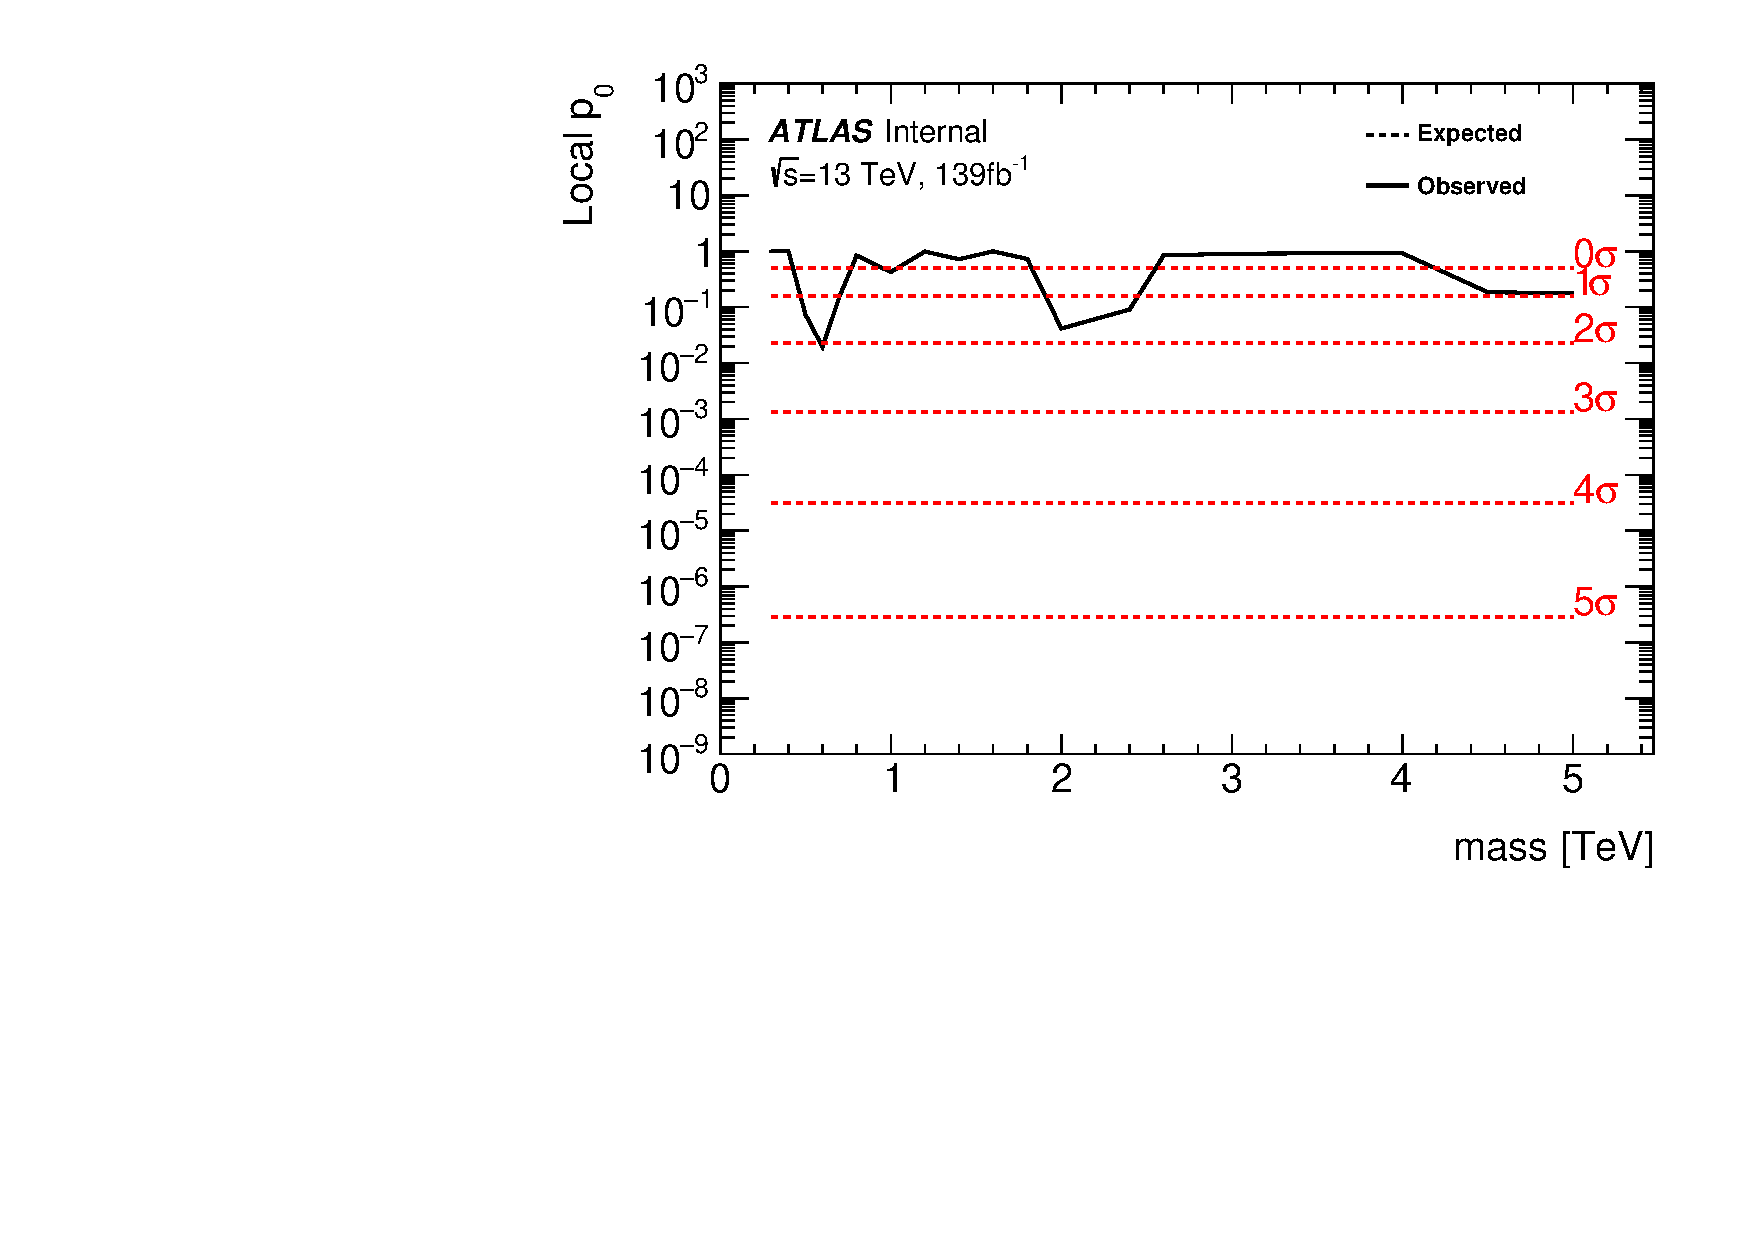
\includegraphics[width=\hsize]{figures/results/pvalues/fixed_pvalues/hvtww_pvalue.pdf}
 \caption{These plots show the measured $p_{0}$ value as a function of resonance mass for HVT Z' DY production.} 
  \label{fig:discov_hvtww}
\end{figure} 
\FloatBarrier

\begin{figure}[h!]
  \centering
  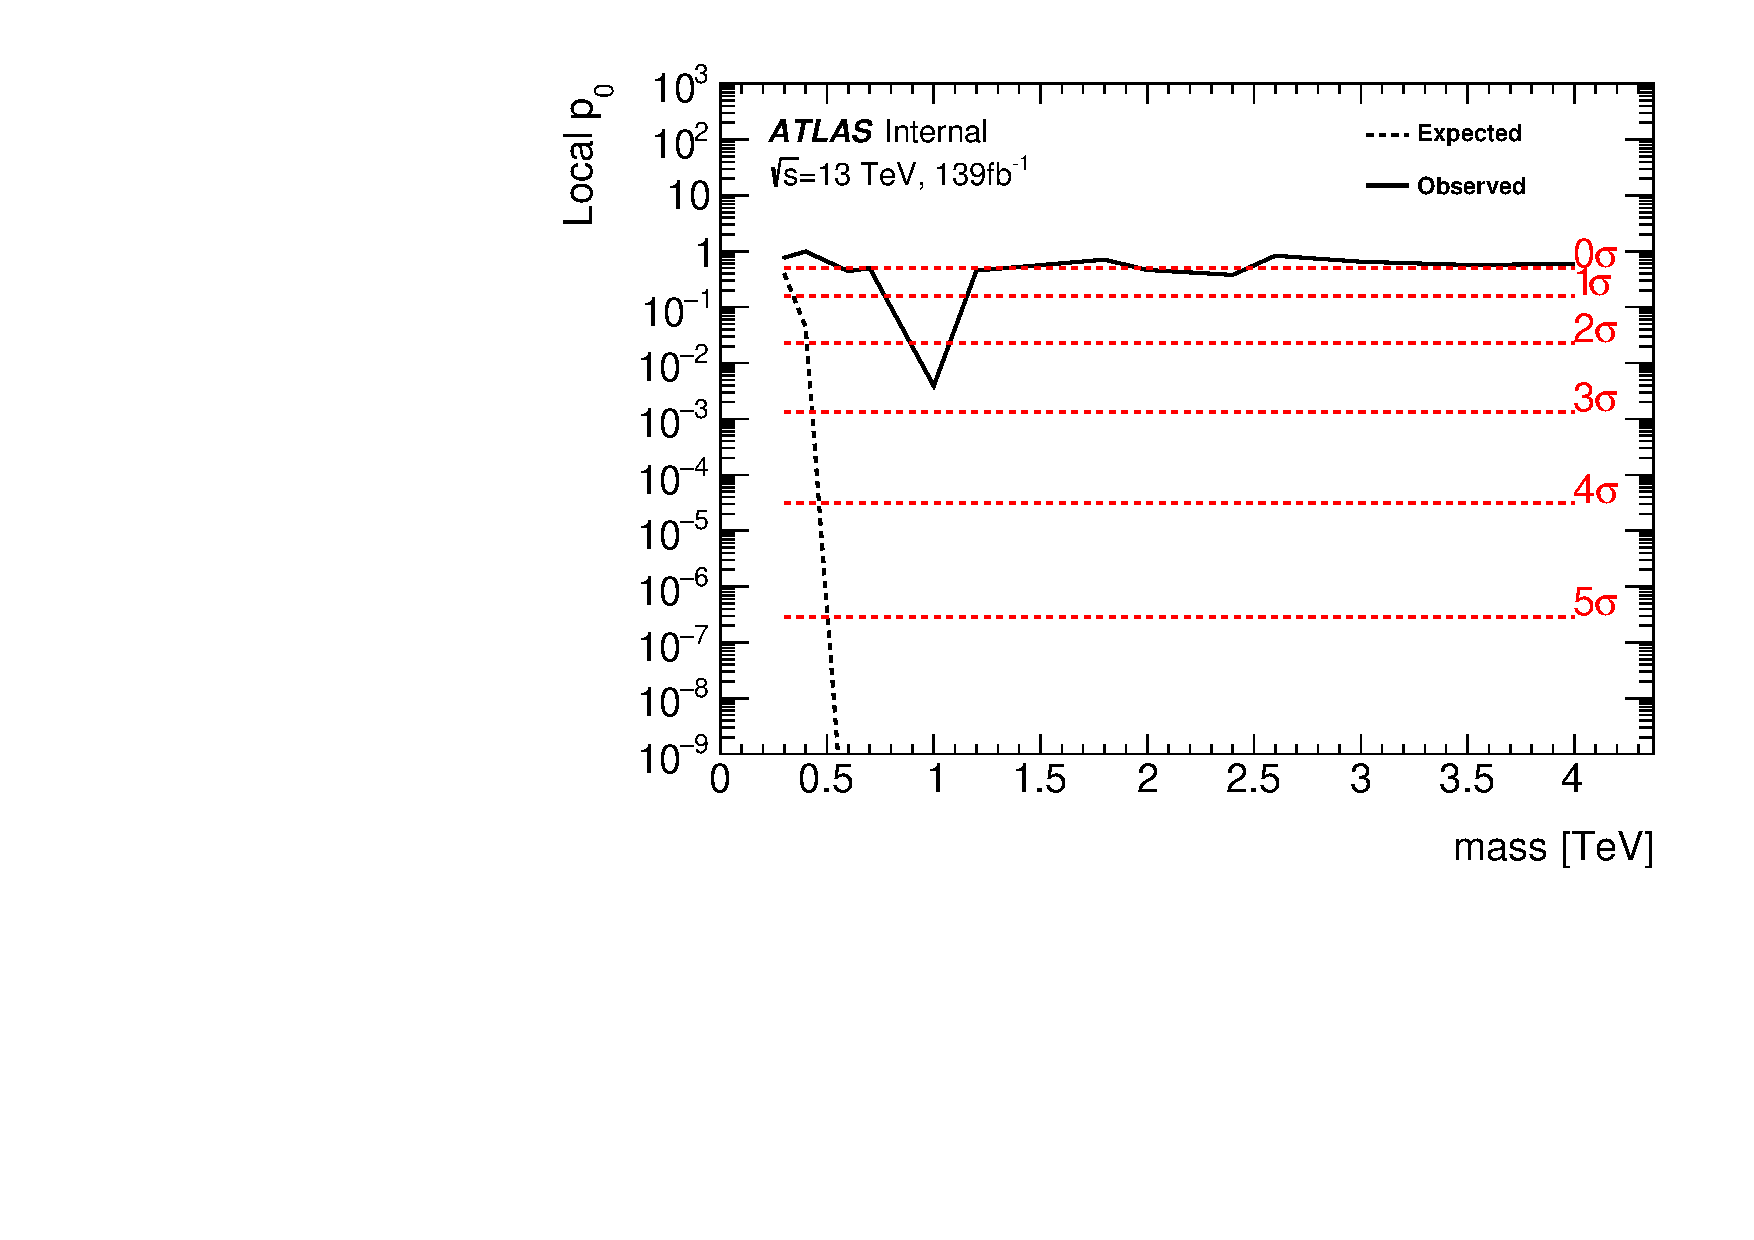
\includegraphics[width=\hsize]{figures/results/pvalues/fixed_pvalues/hvtwwvbf_pvalue.pdf}
 \caption{These plots show the measured $p_{0}$ value as a function of resonance mass for HVT Z' VBF production.} 
  \label{fig:discov_hvtwwvbf}
\end{figure} 
\FloatBarrier


\begin{figure}[h!]
  \centering
  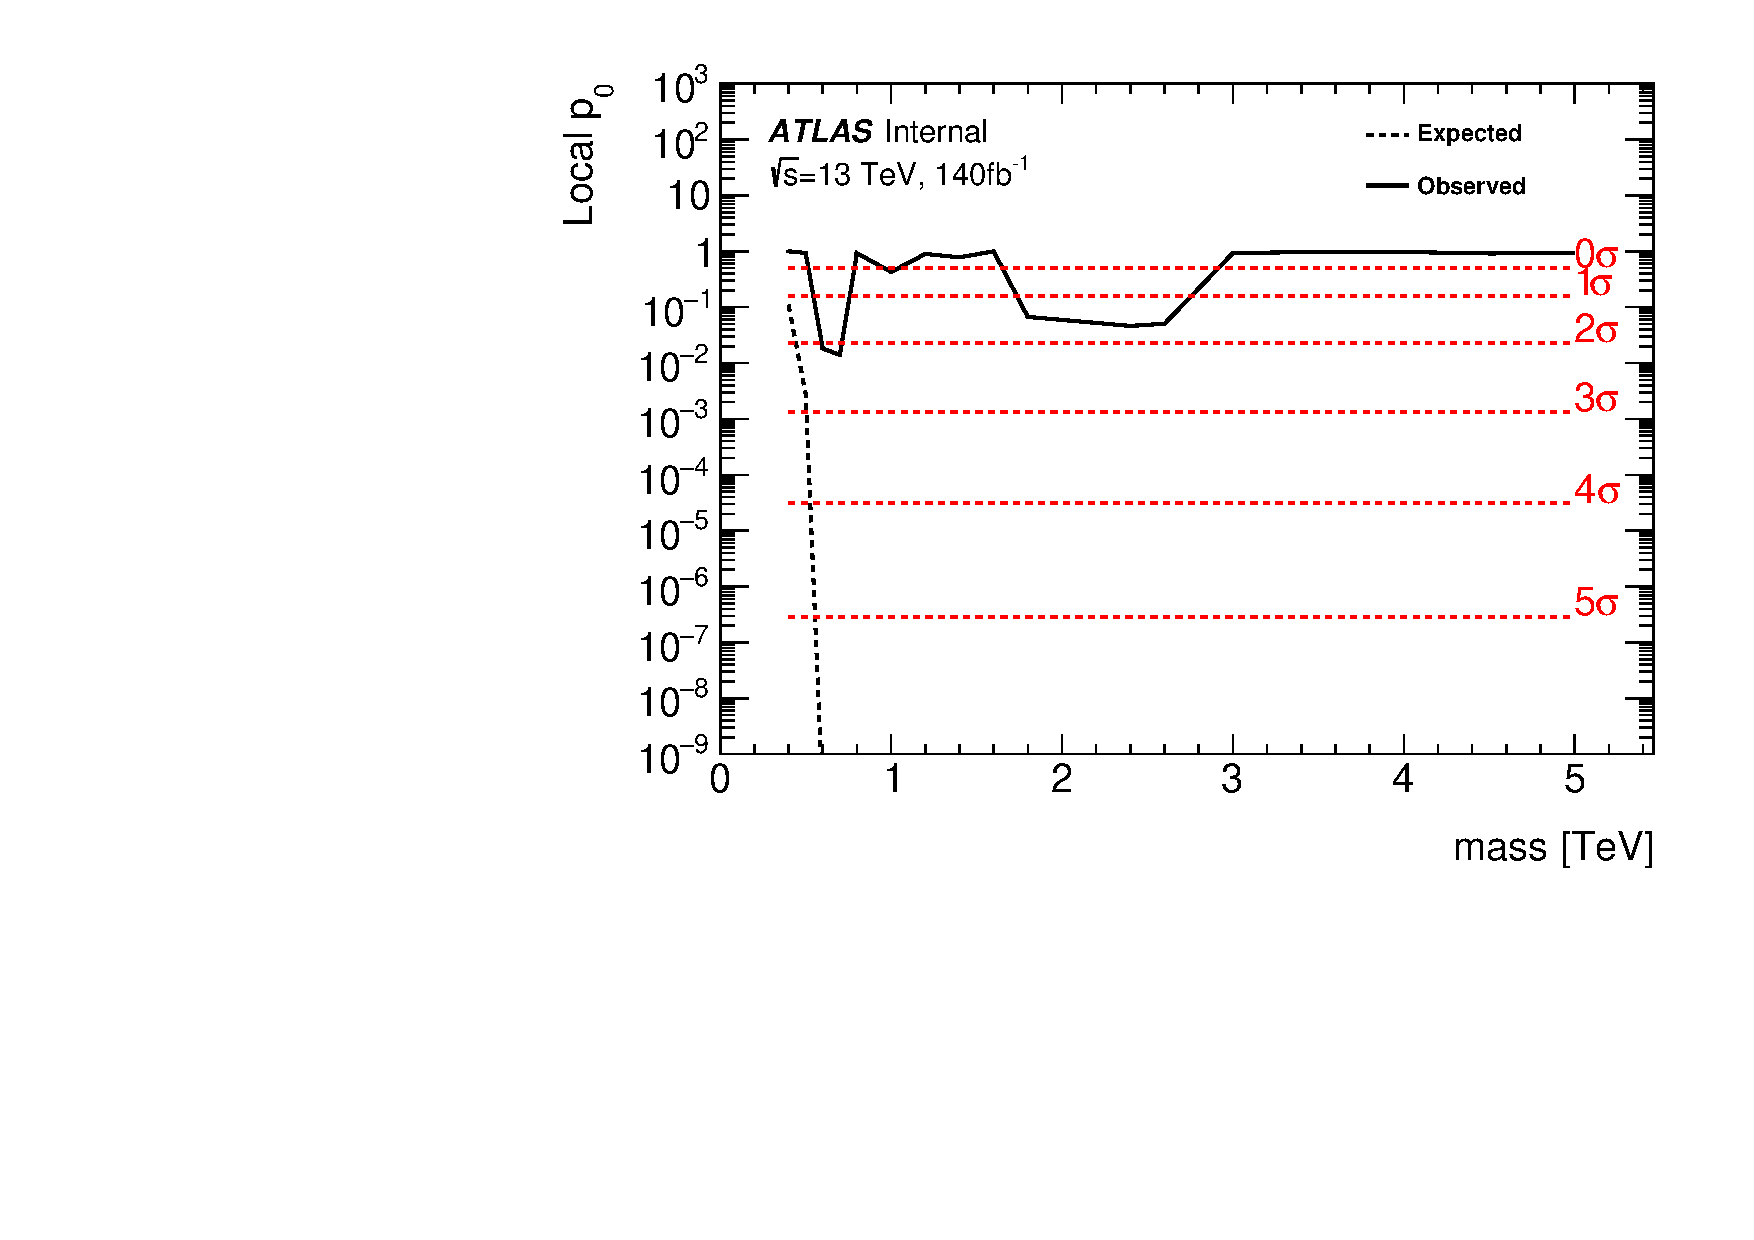
\includegraphics[width=\hsize]{figures/results/pvalues/fixed_pvalues/hvtwz_pvalue.pdf}
 \caption{These plots show the measured $p_{0}$ value as a function of resonance mass for HVT W' DY production.} 
  \label{fig:discov_hvtwz}
\end{figure} 
\FloatBarrier

\begin{figure}[h!]
  \centering
  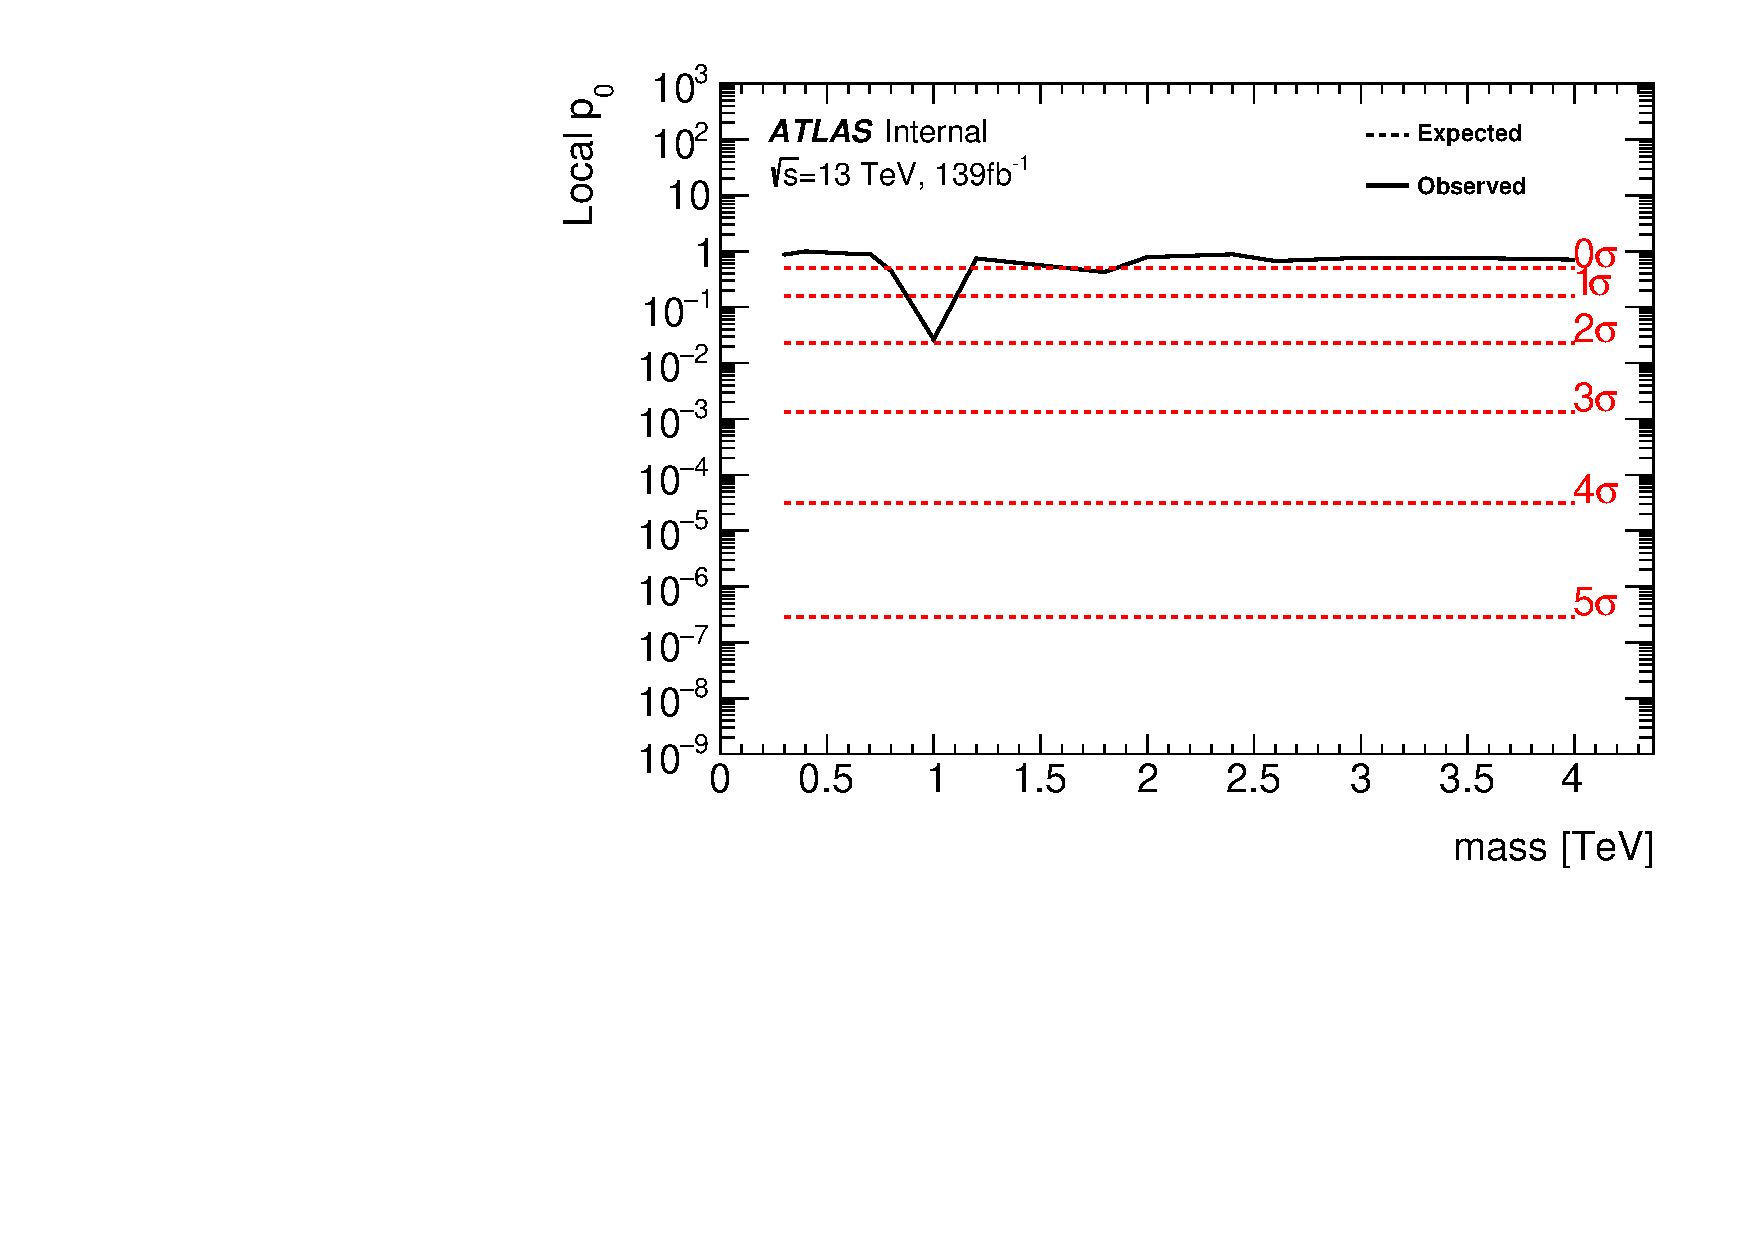
\includegraphics[width=\hsize]{figures/results/pvalues/fixed_pvalues/hvtwzvbf_pvalue.pdf}
 \caption{These plots show the measured $p_{0}$ value as a function of resonance mass for HVT W' VBF production.} 
  \label{fig:discov_hvtwzvbf}
\end{figure} 
\FloatBarrier


\begin{figure}[h!]
  \centering
  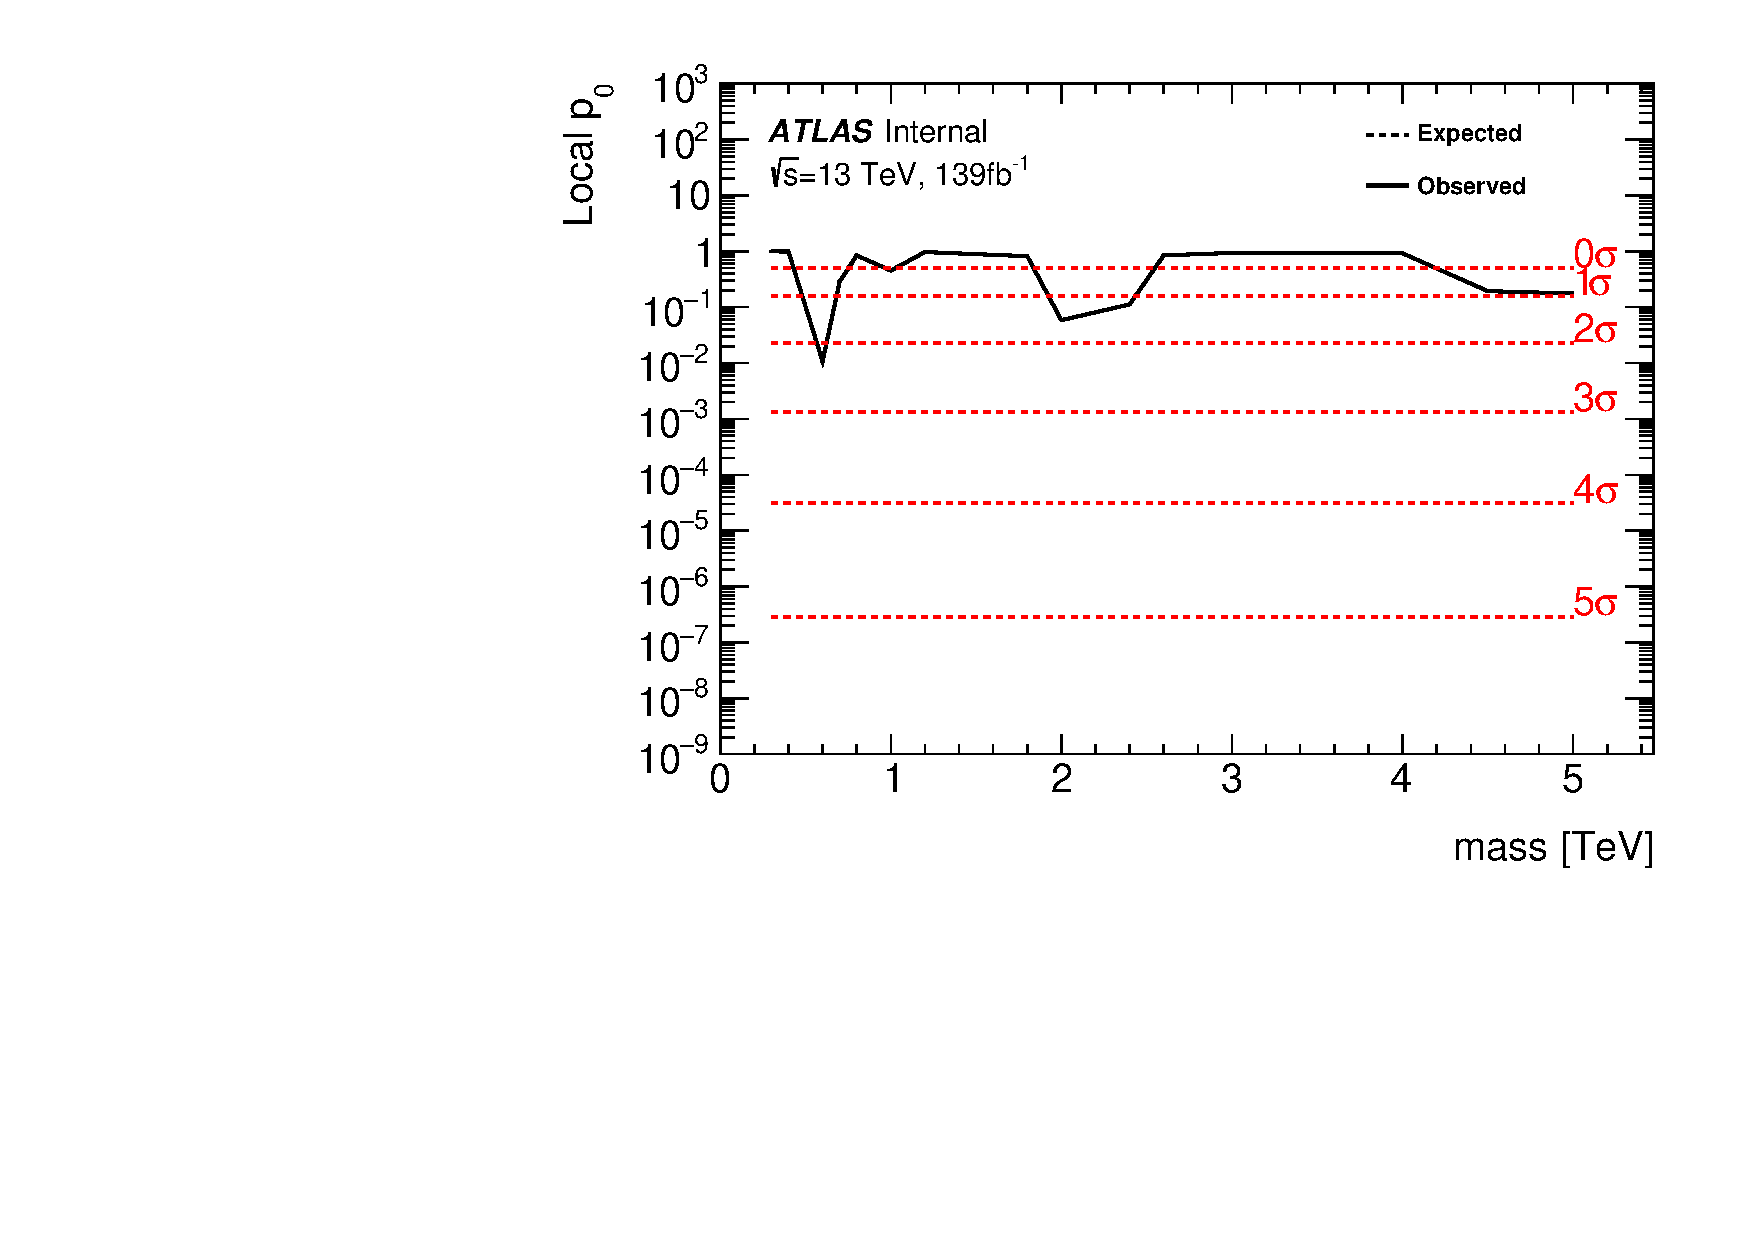
\includegraphics[width=\hsize]{figures/results/pvalues/fixed_pvalues/rsg_pvalue.pdf}
 \caption{These plots show the measured $p_{0}$ value as a function of resonance mass for the RS Graviton ggF production.} 
  \label{fig:discov_rsg}
\end{figure} 
\FloatBarrier


\section{Limits}
Using the exclusion limits tests discussed previously, exclusion limits are set on $\mu$ and consequently cross-sections for different signal models. Exclusion limits for the models considered are shown in Figure \ref{fig:hvtww_limit} - \ref{fig:rsg_limit}. These plots show the theory cross section for a given resonance to decay to $WW/WZ$. Also, an Asimov dataset is used to calculate the limits that could be set for the background only hypothesis with the associated errors on this predictions. Finally, the observed limits are shown in black. All signal mass where the theory prediction is less than the observed prediction are excluded at the 95\% confidence level. These limits shown exclude HVT Model A W' $< 3.4$ TeV and Z' $< 3.3$ TeV and Model B W' $< 3.7$ TeV and Z'$ < 3.7$ TeV. Randall Sundrum Gravitons are excluded for masses below 1.6TeV .


\begin{figure}[h!]
  \centering
  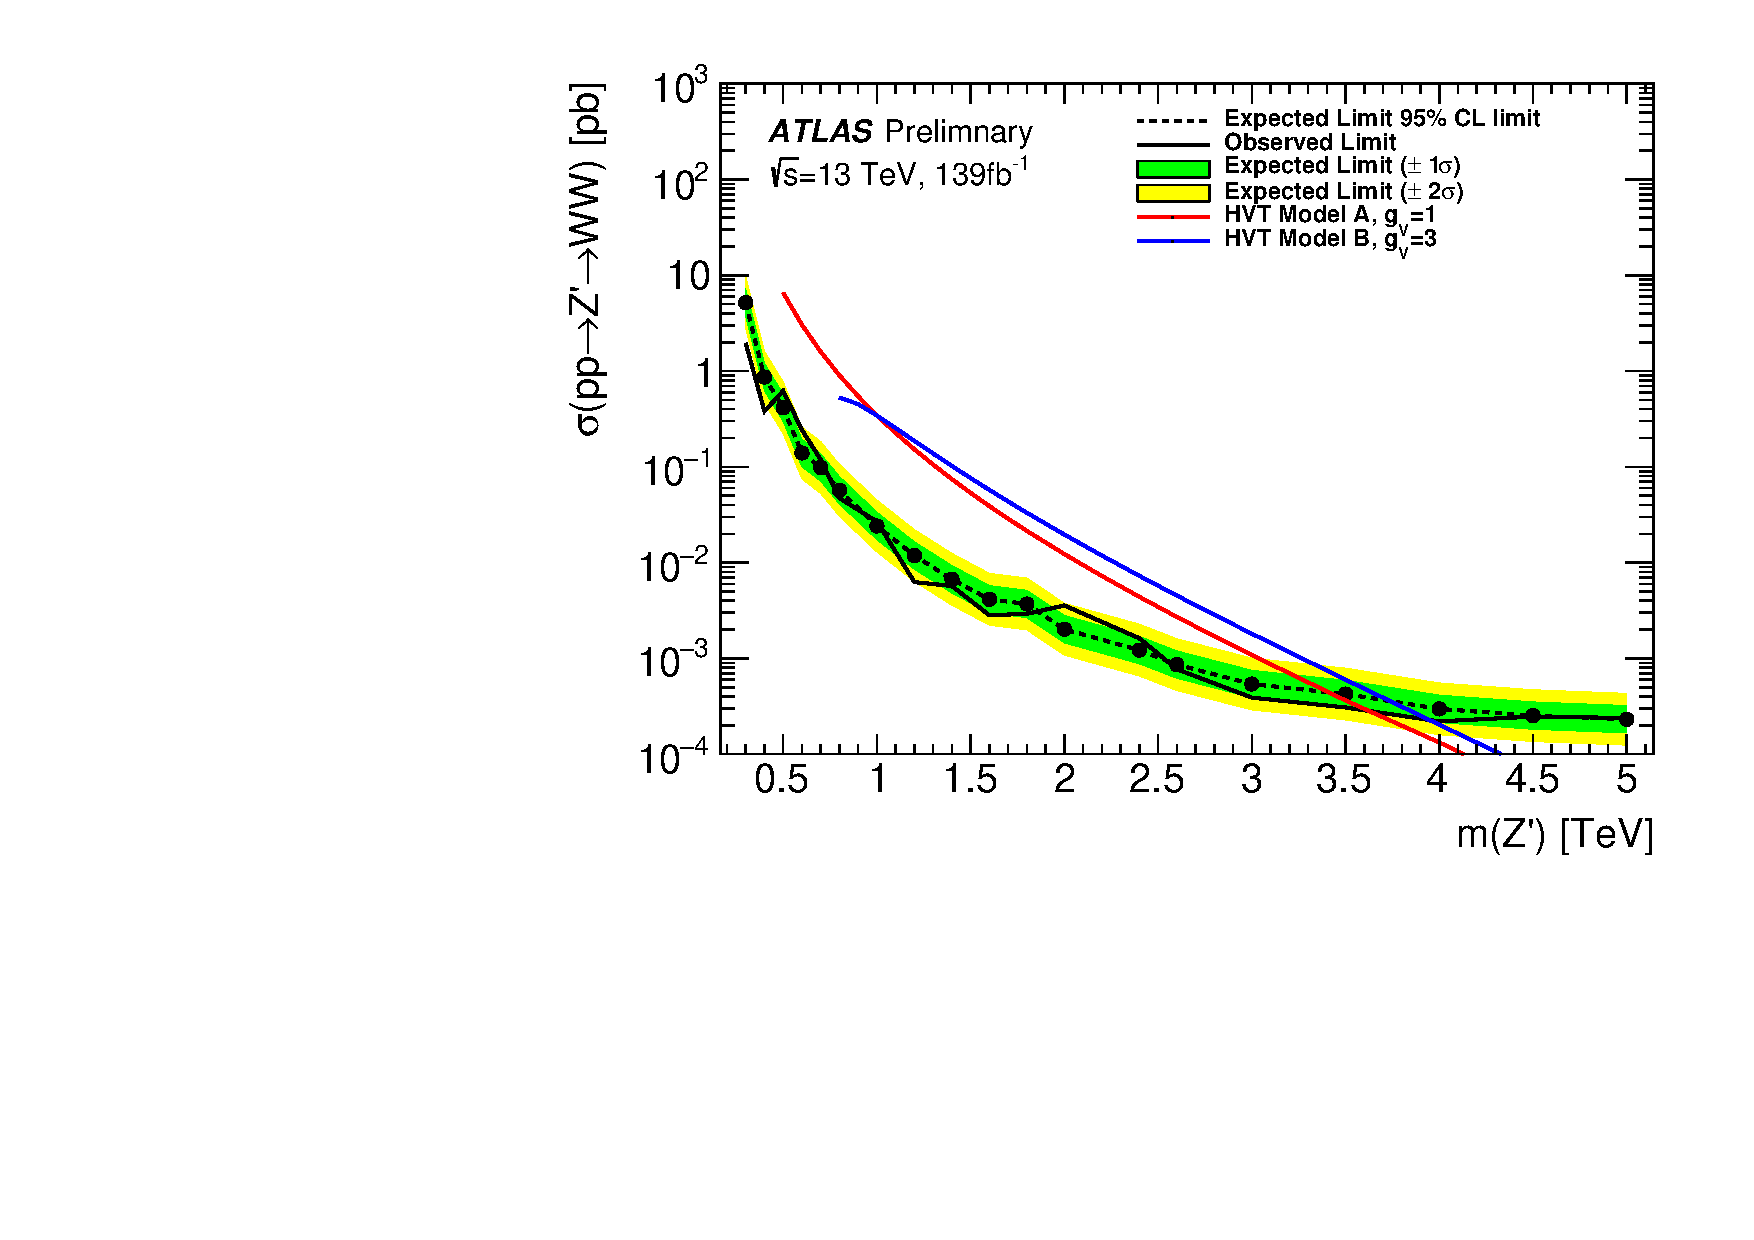
\includegraphics[width=0.48\hsize]{figures/results/limits/limits_hvtww.pdf}
  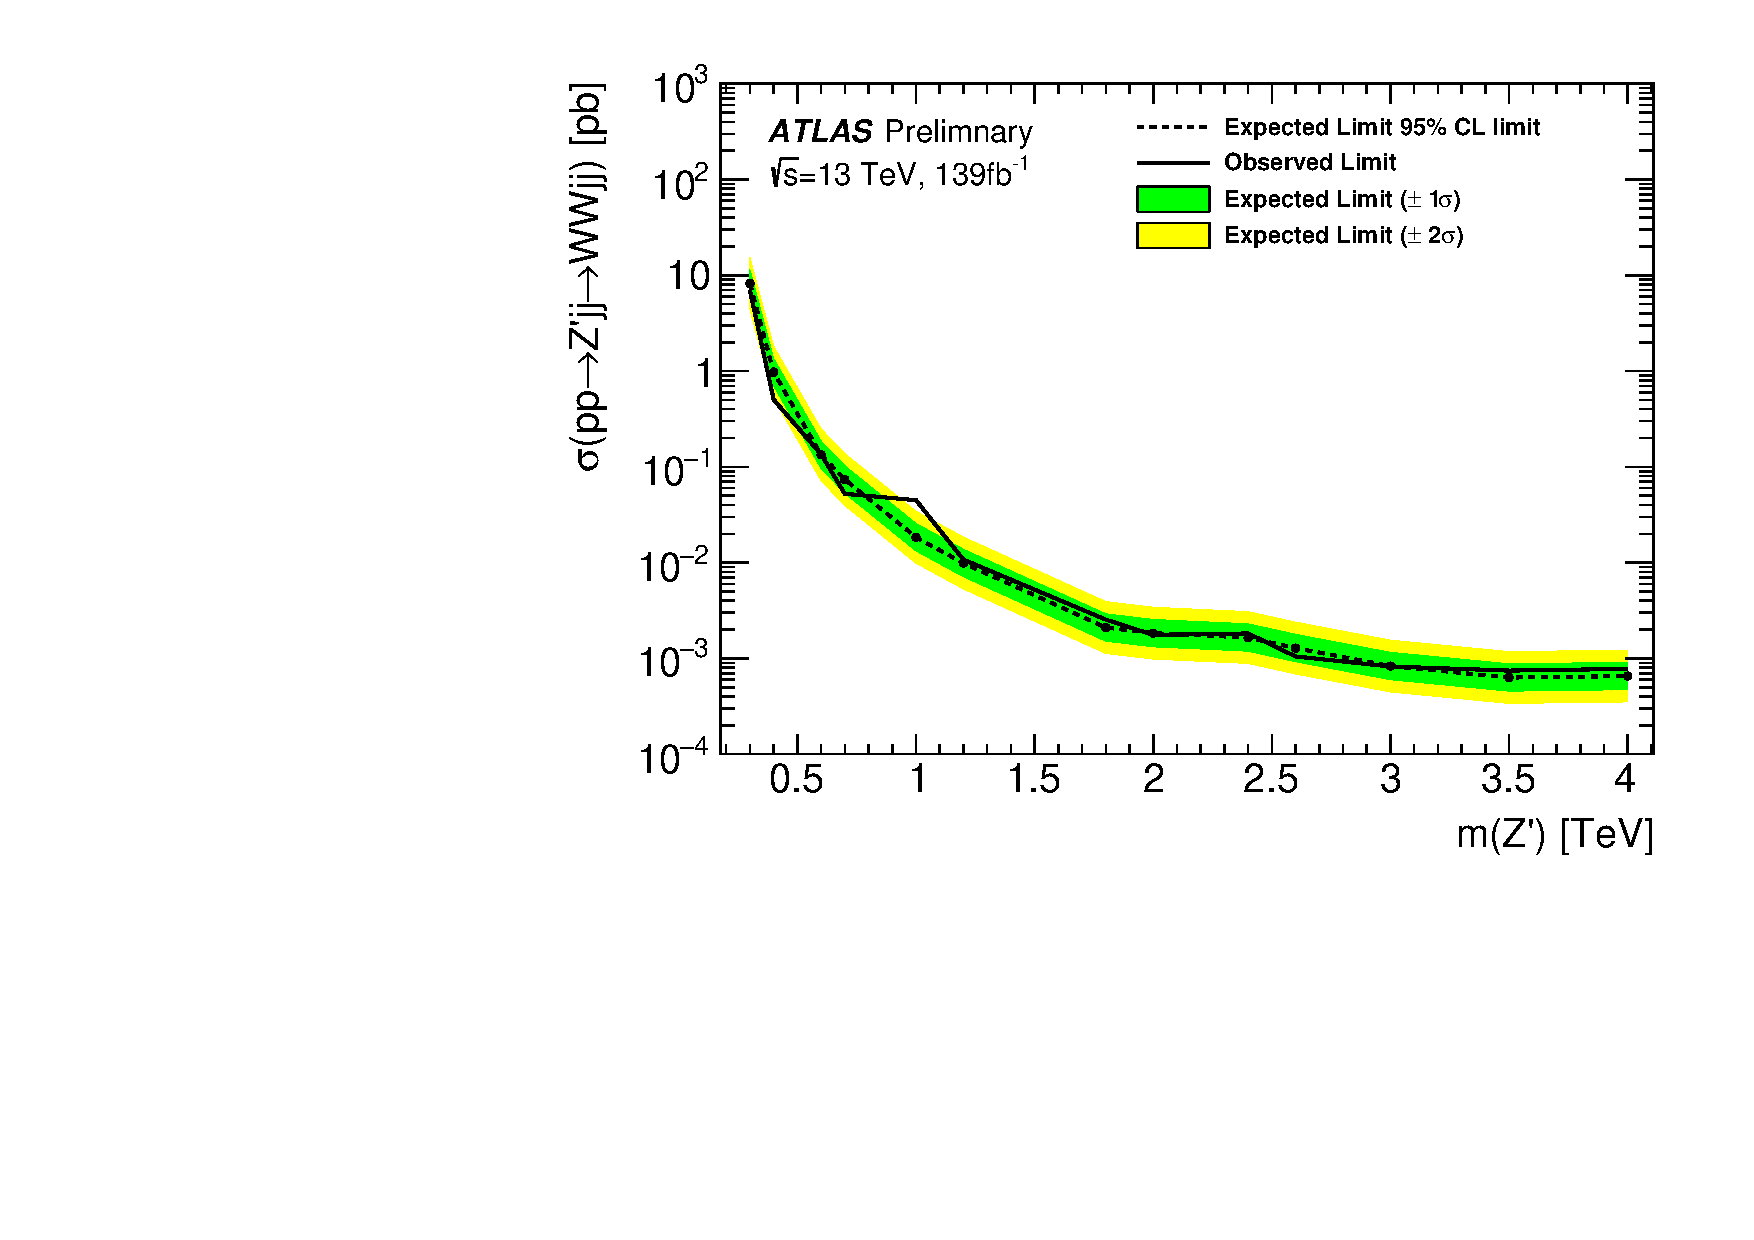
\includegraphics[width=0.48\hsize]{figures/results/limits/limits_hvtwwvbf.pdf}

 \caption{Theory, expected and observed limits for HVT $W'$ DY (left) and VBF (right) production.}
  \label{fig:hvtww_limit}
\end{figure} 
\FloatBarrier


\begin{figure}[h!]
  \centering
  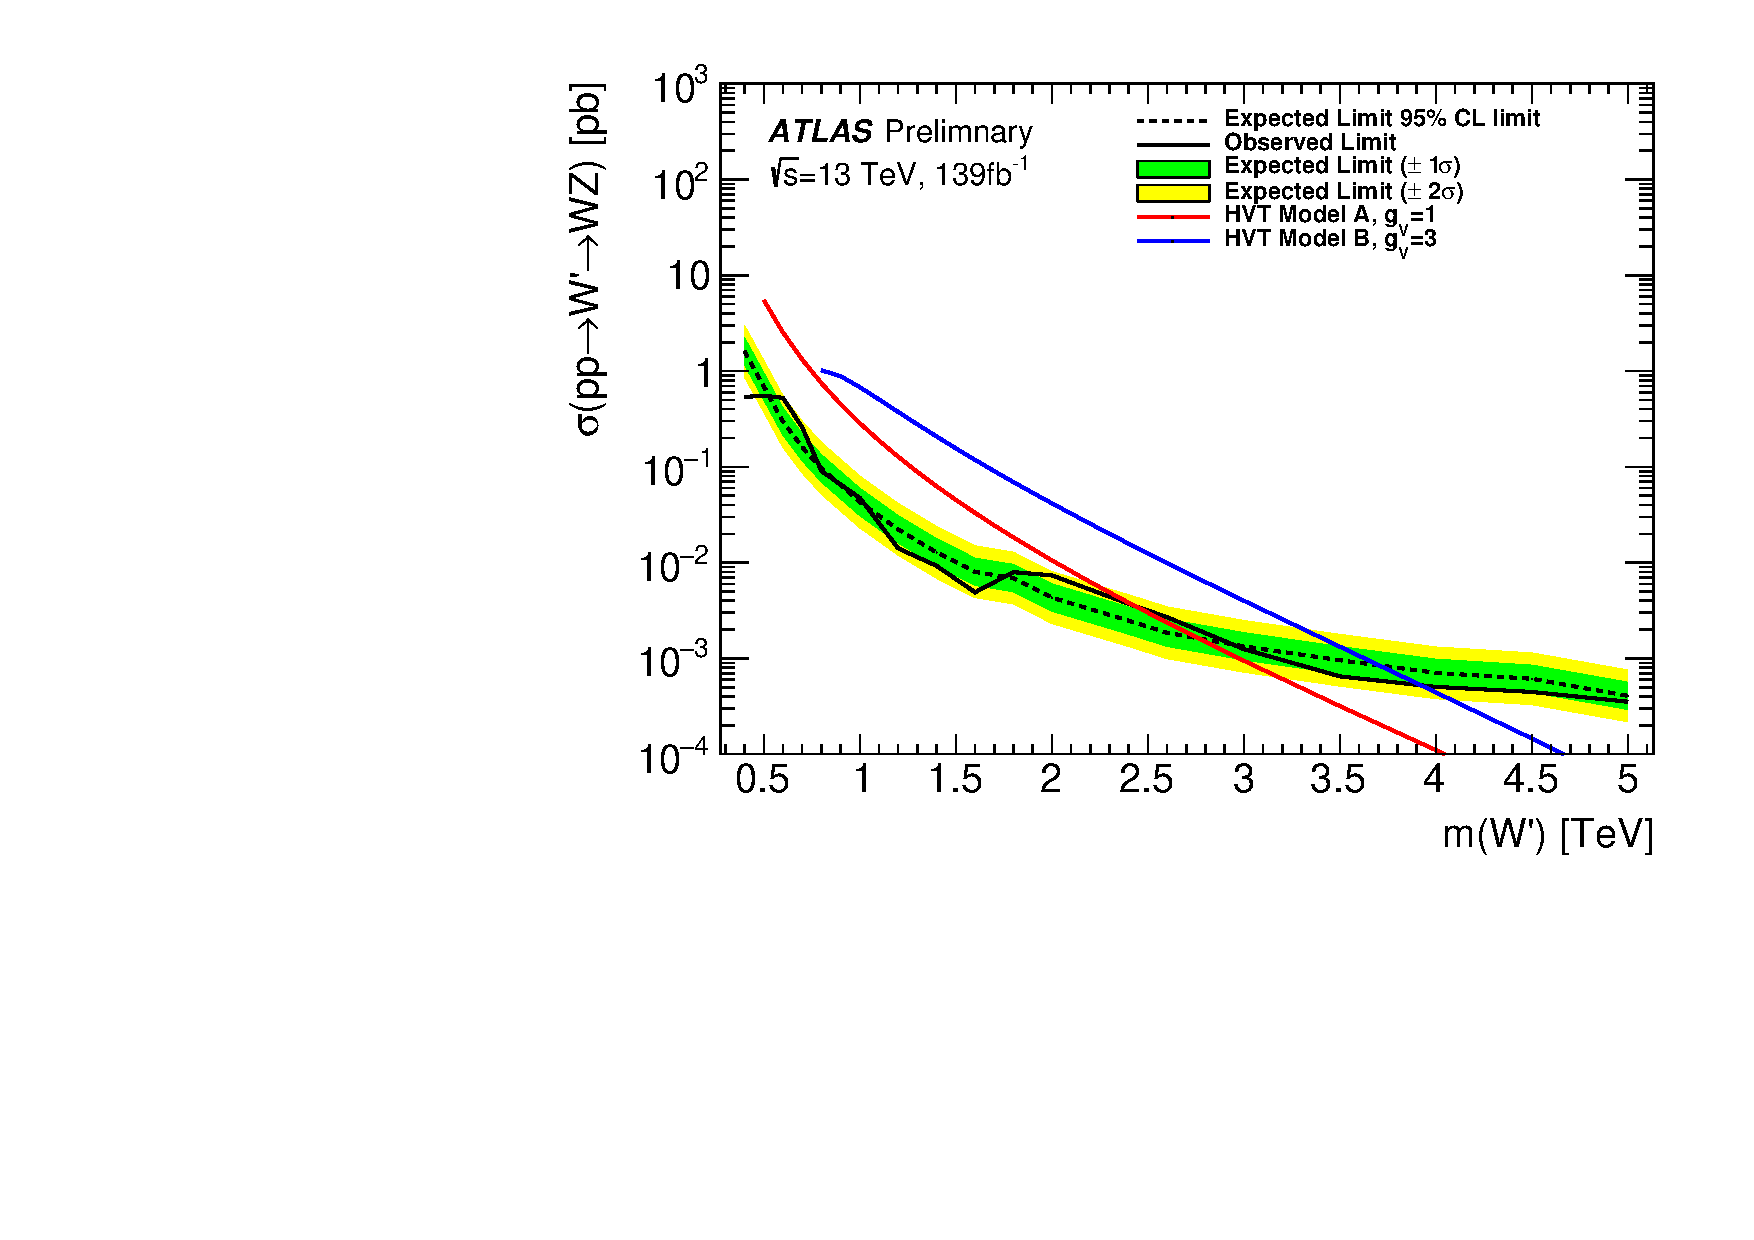
\includegraphics[width=0.48\hsize]{figures/results/limits/limits_hvtwz.pdf}
  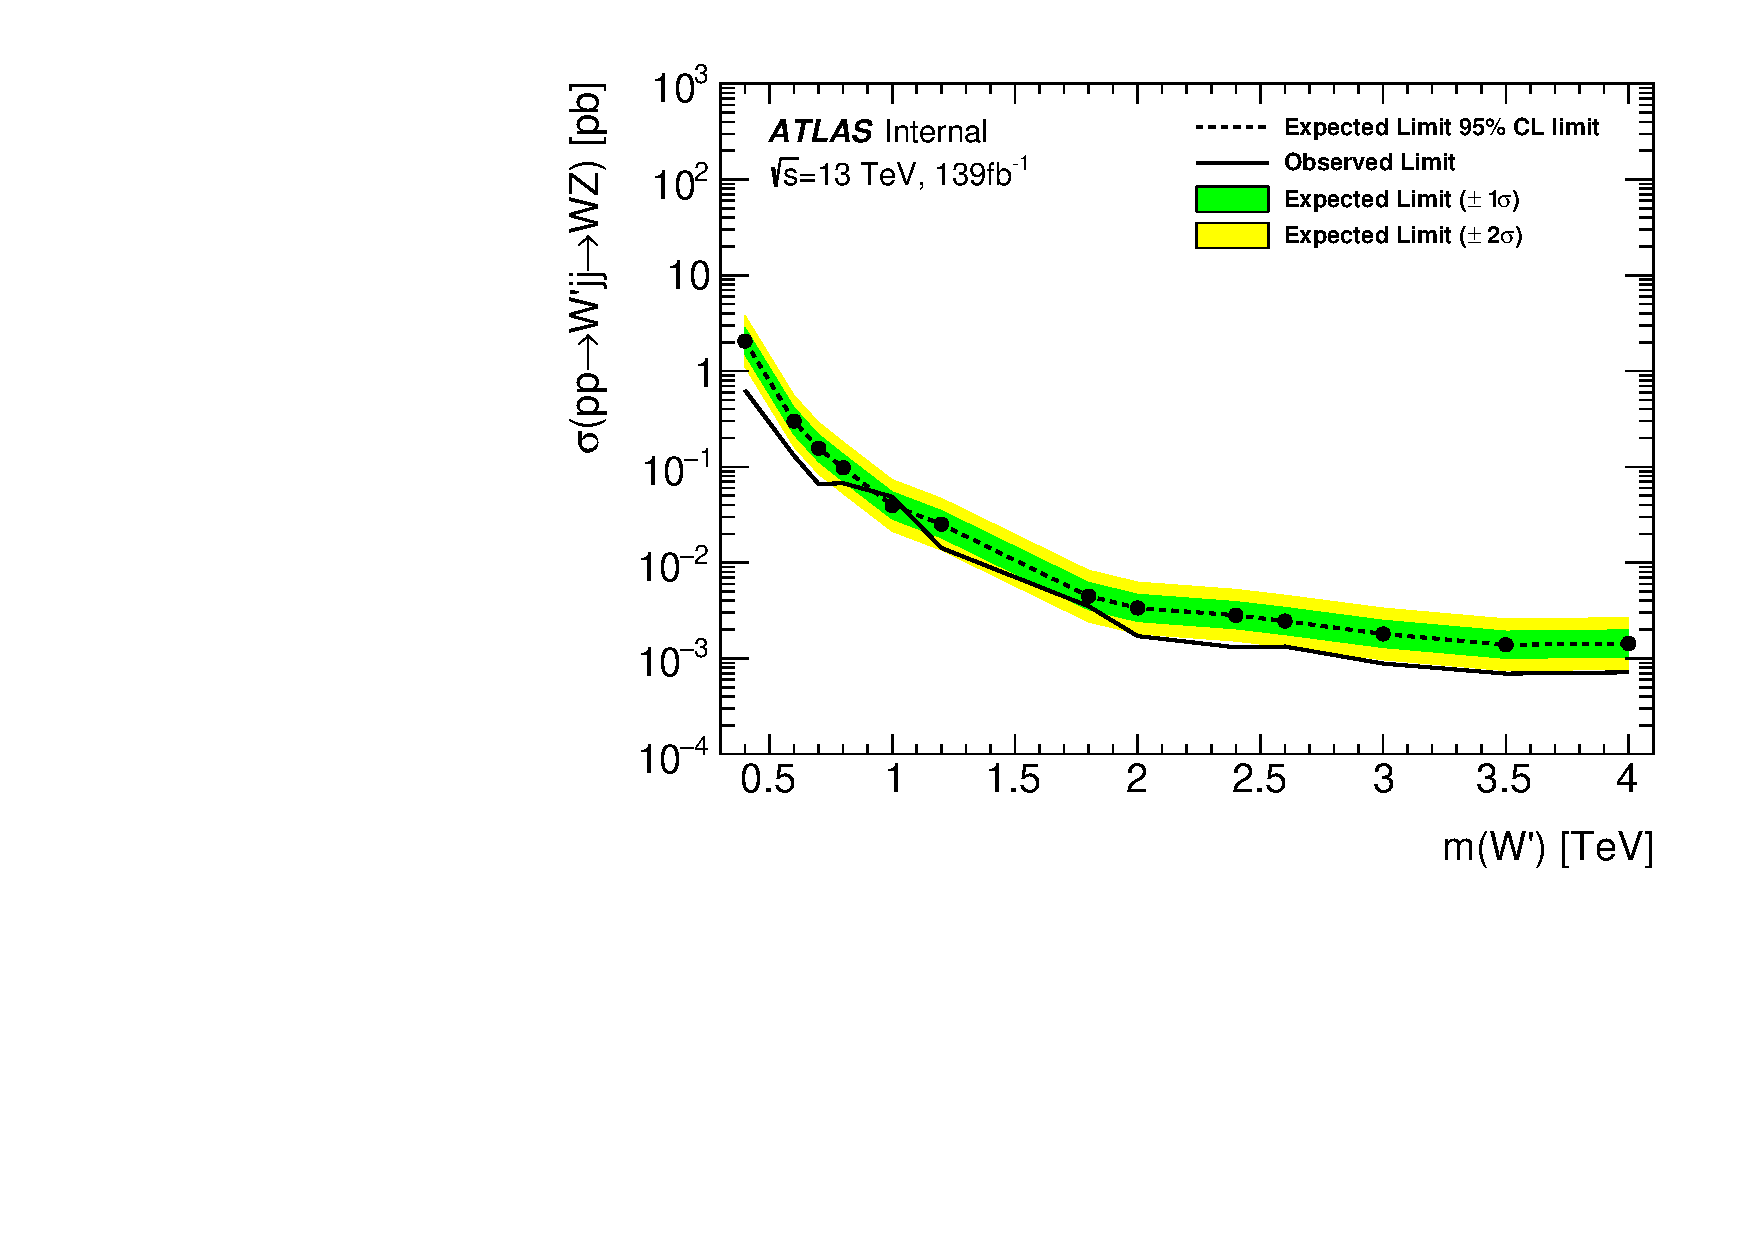
\includegraphics[width=0.48\hsize]{figures/results/limits/limits_hvtwzvbf.pdf}

 \caption{Theory, expected and observed limits for HVT $Z'$ DY (left) and VBF (right) production.}
  \label{fig:hvtwz_limit}
\end{figure} 
\FloatBarrier

\begin{figure}[h!]
  \centering
  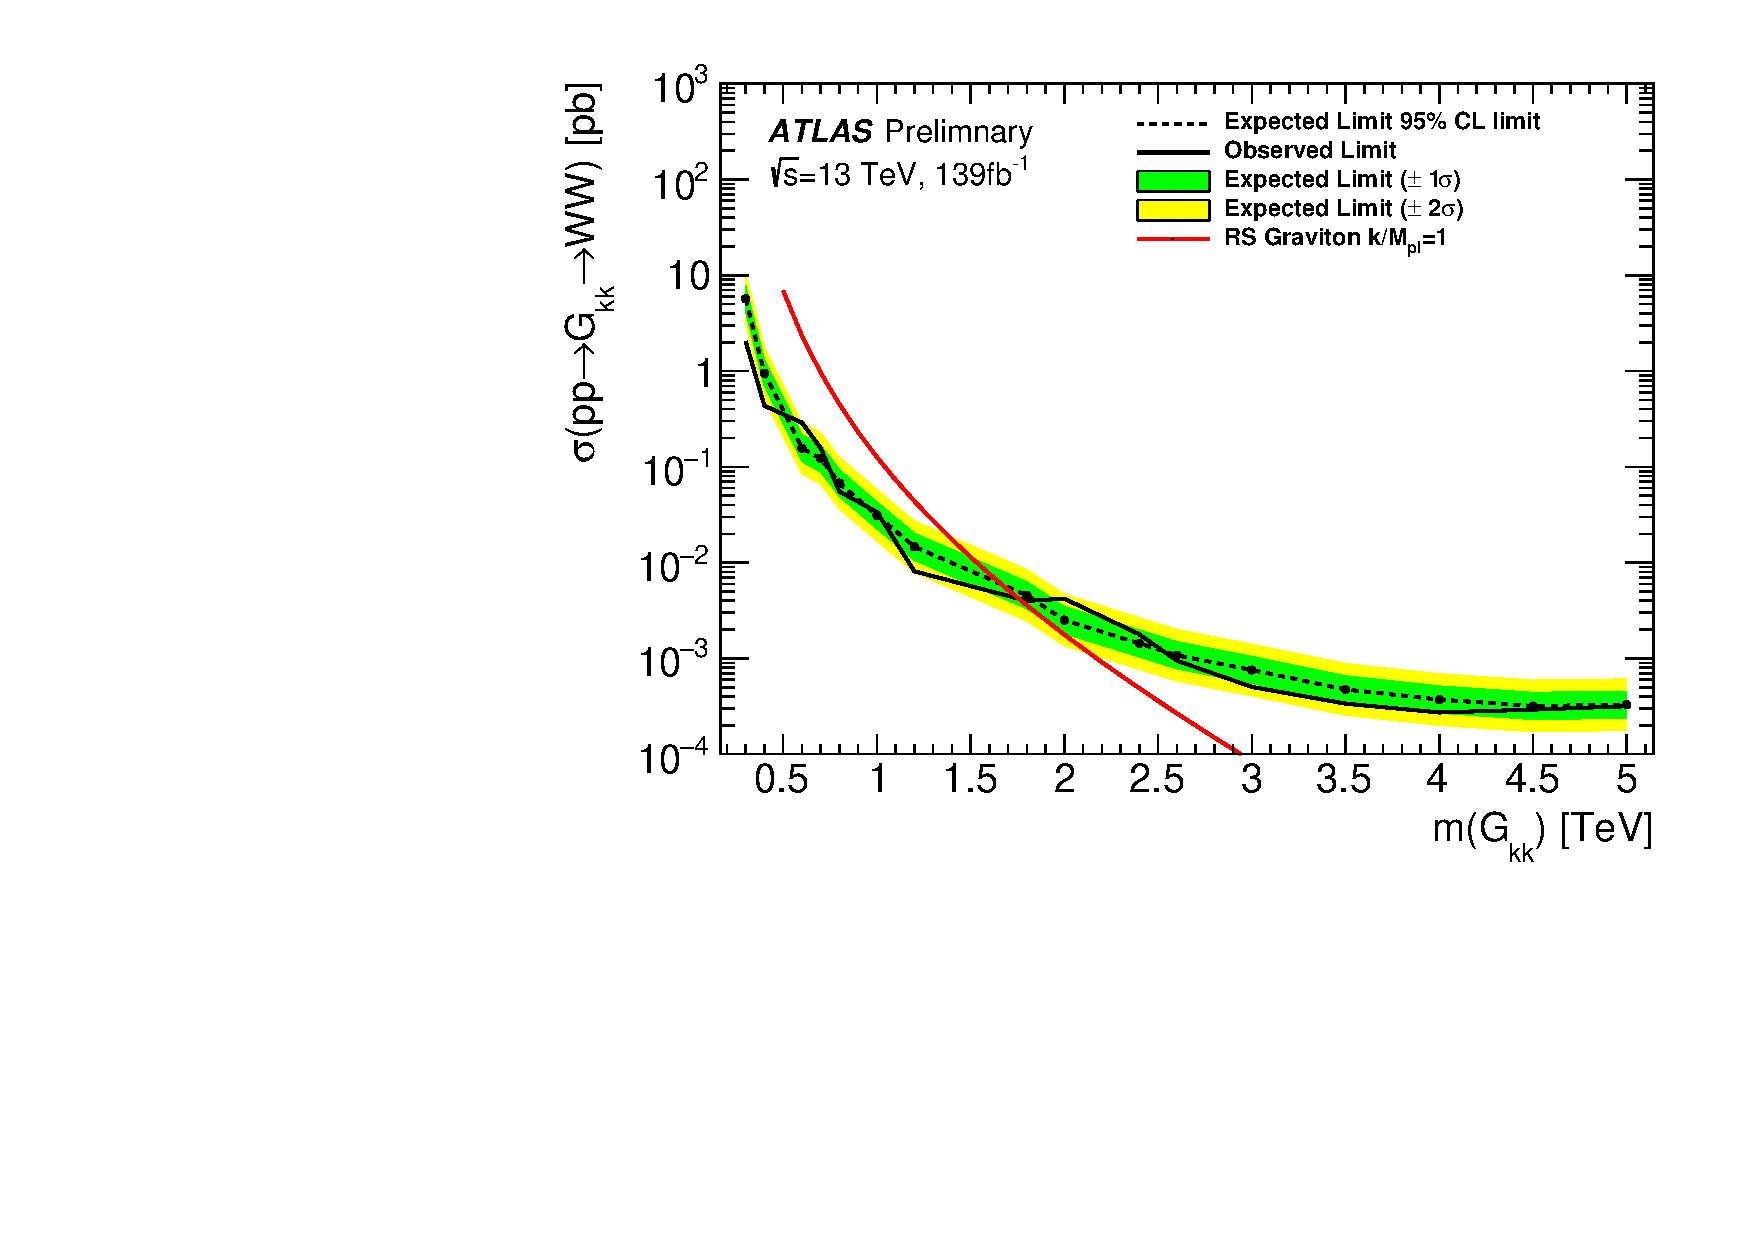
\includegraphics[width=\hsize]{figures/results/limits/limits_rsg.pdf}

 \caption{Theory, expected and observed limits for RS Gravitons via gluon-gluon fusion production.}
  \label{fig:rsg_limit}
\end{figure} 
\FloatBarrier
